\documentclass[../SustainableHEP.tex]{subfiles}
\begin{document}
\RaggedRight
\sloppy
\newpage

%%%%%%%%%%%%%%%%%%%%%%%%%%%%%%%%%%%%%%%%%%%%%%%%%%

\section{Food}
\label{sec:Food}

\begin{figure}
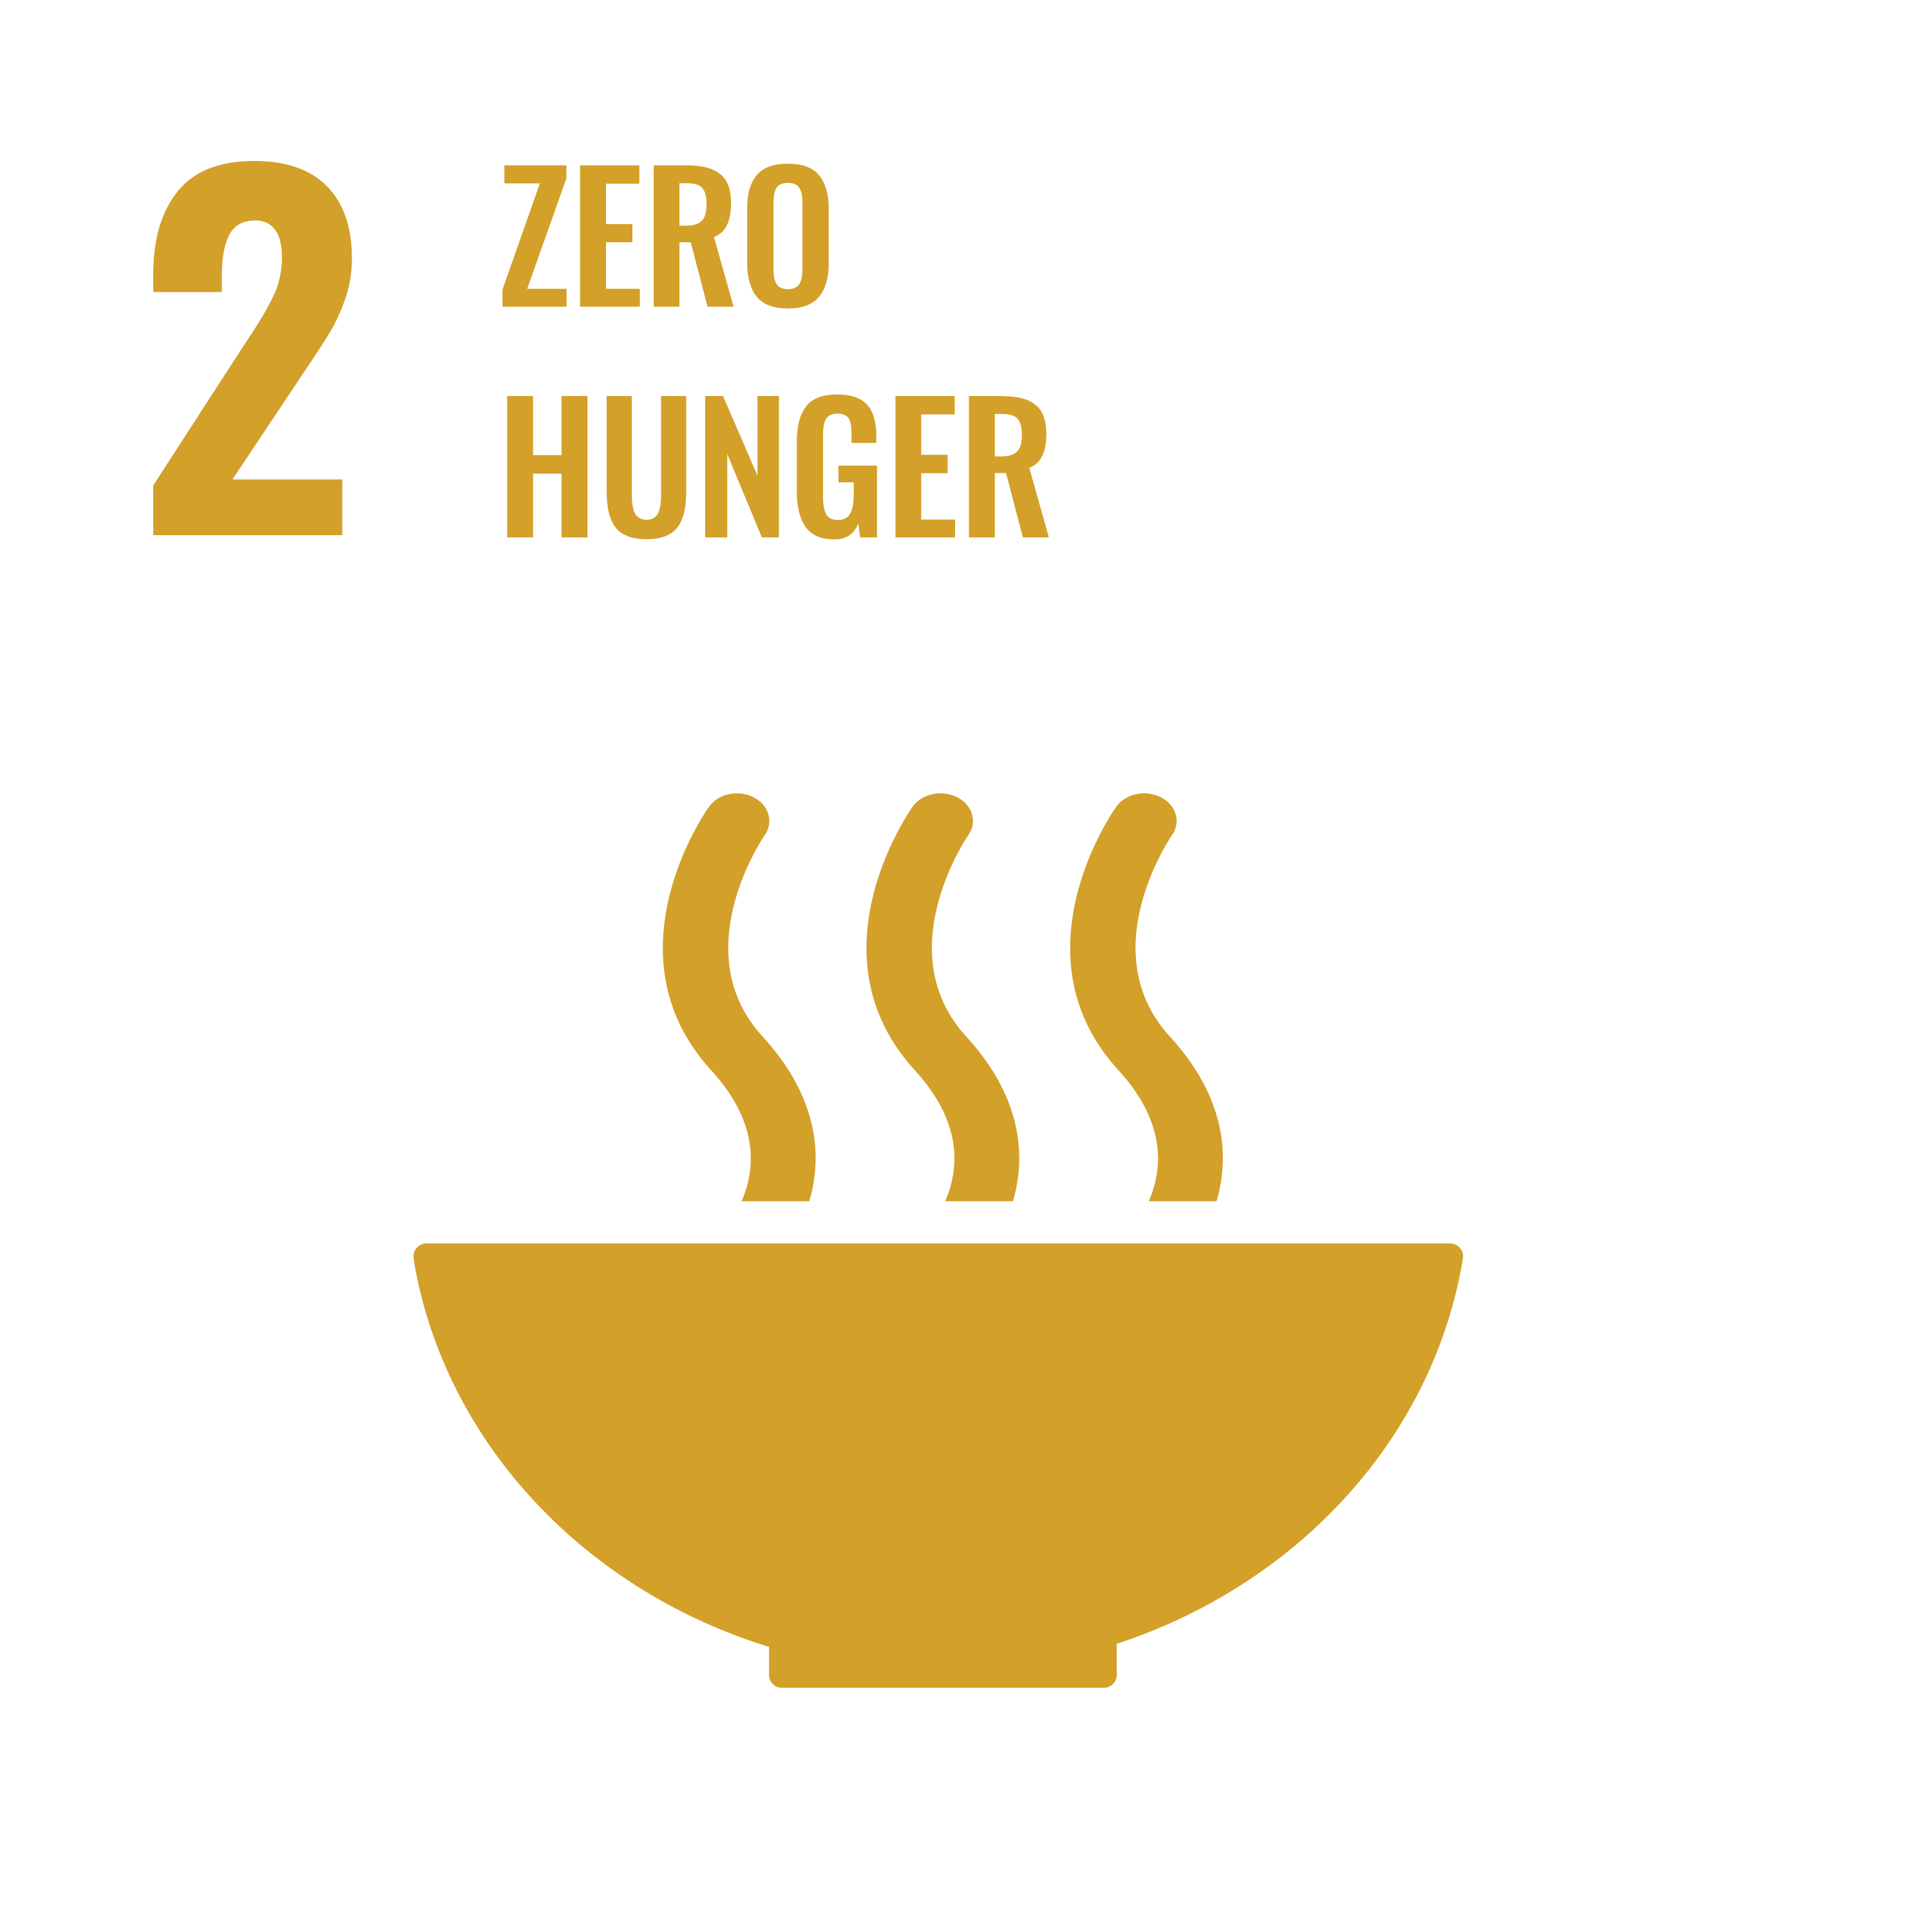
\includegraphics[width=\SDGsize]{Common/SDG_2_ZeroHunger.png}~%
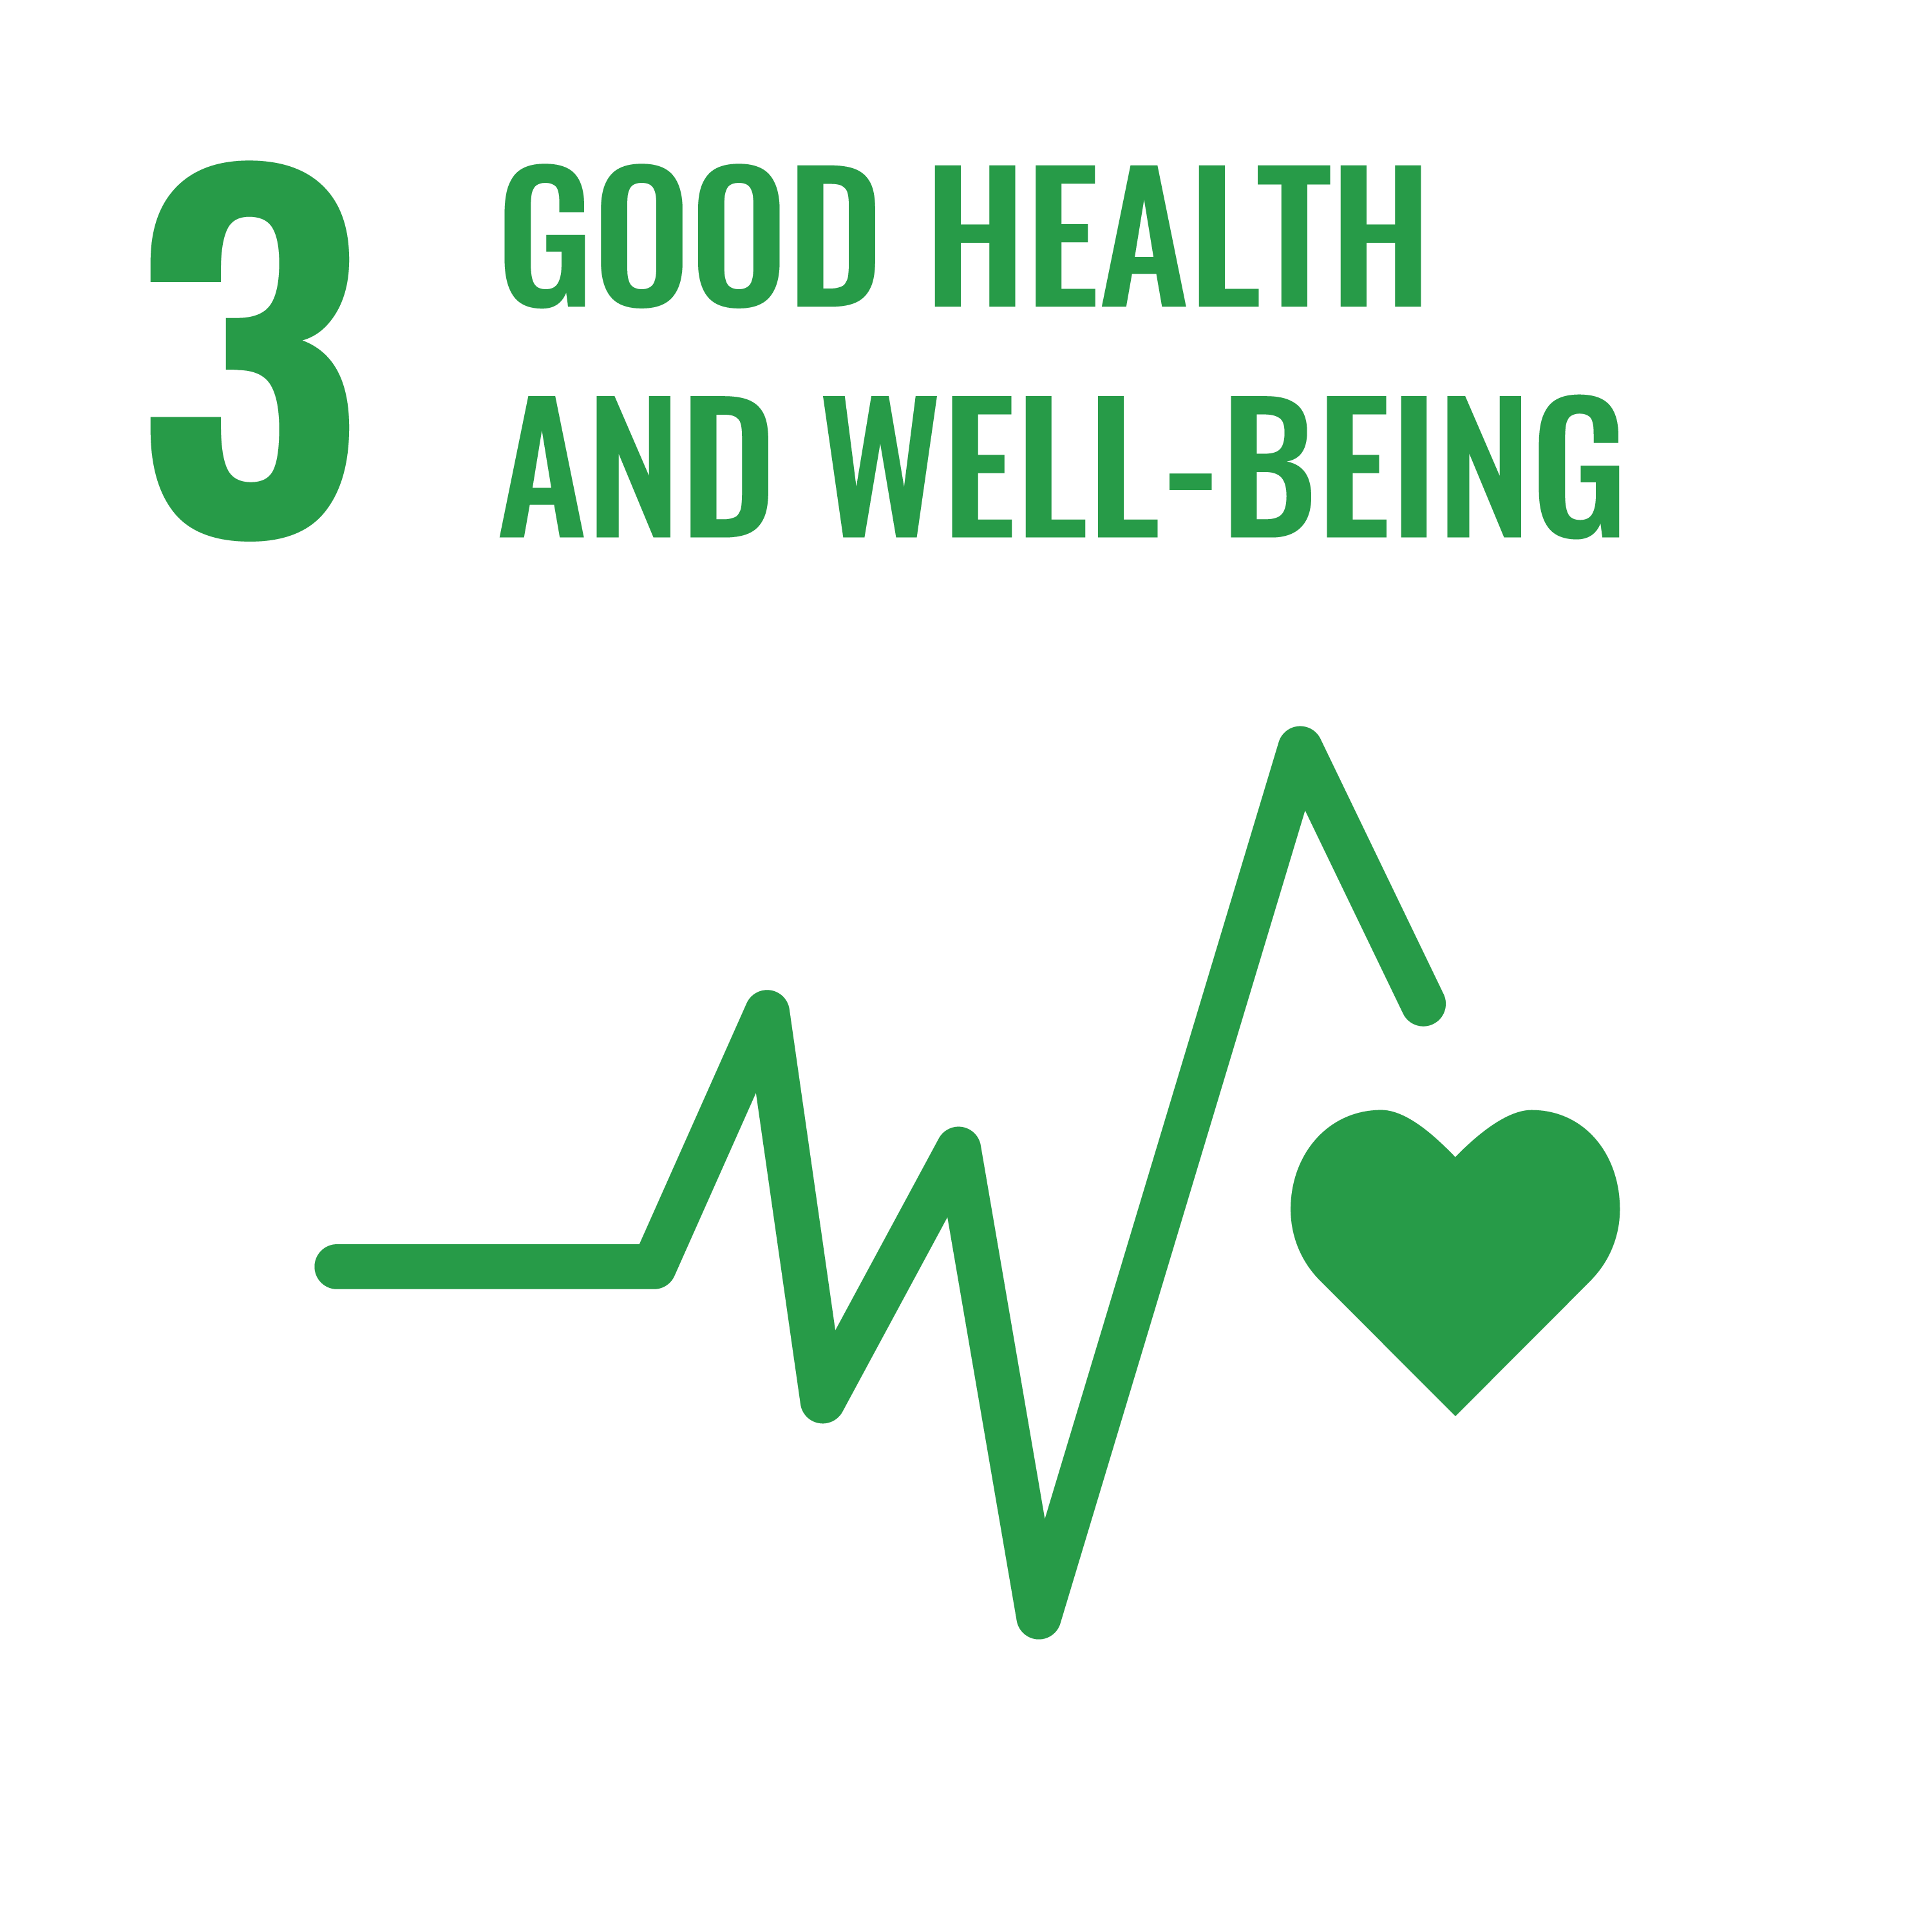
\includegraphics[width=\SDGsize]{Common/SDG_3_GoodHealth.png}~%
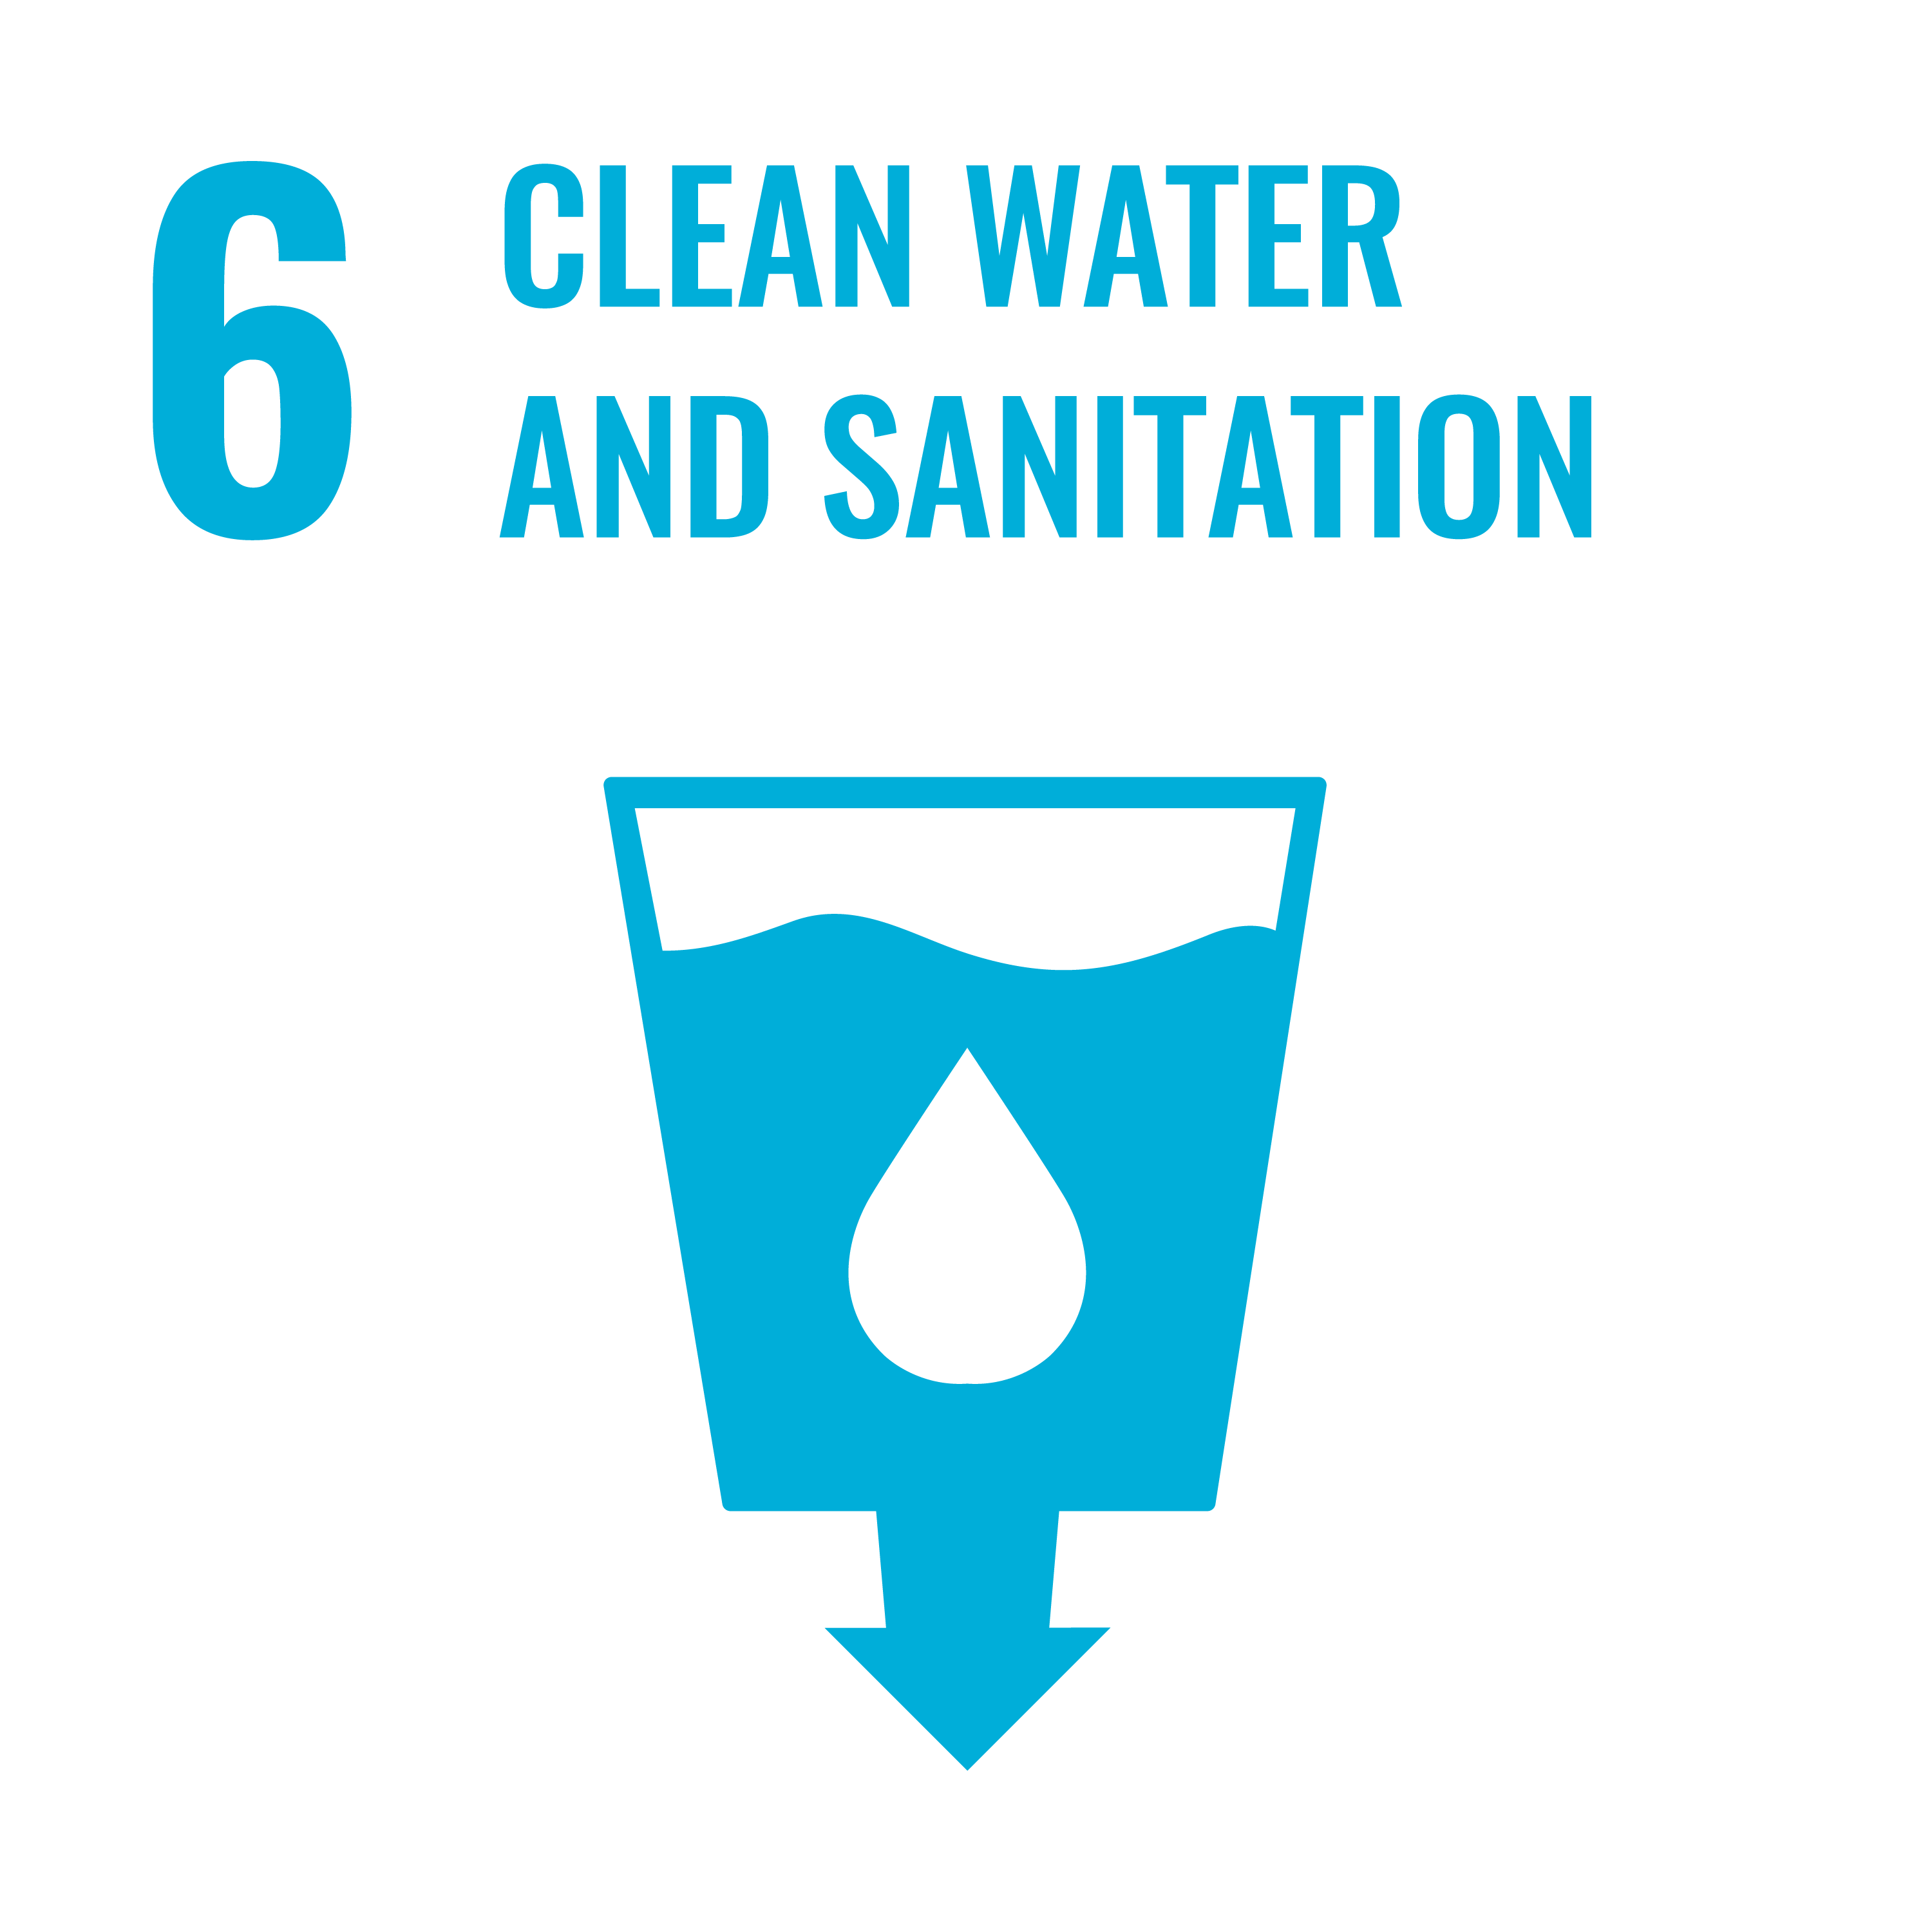
\includegraphics[width=\SDGsize]{Common/SDG_6_CleanWater.png}~%
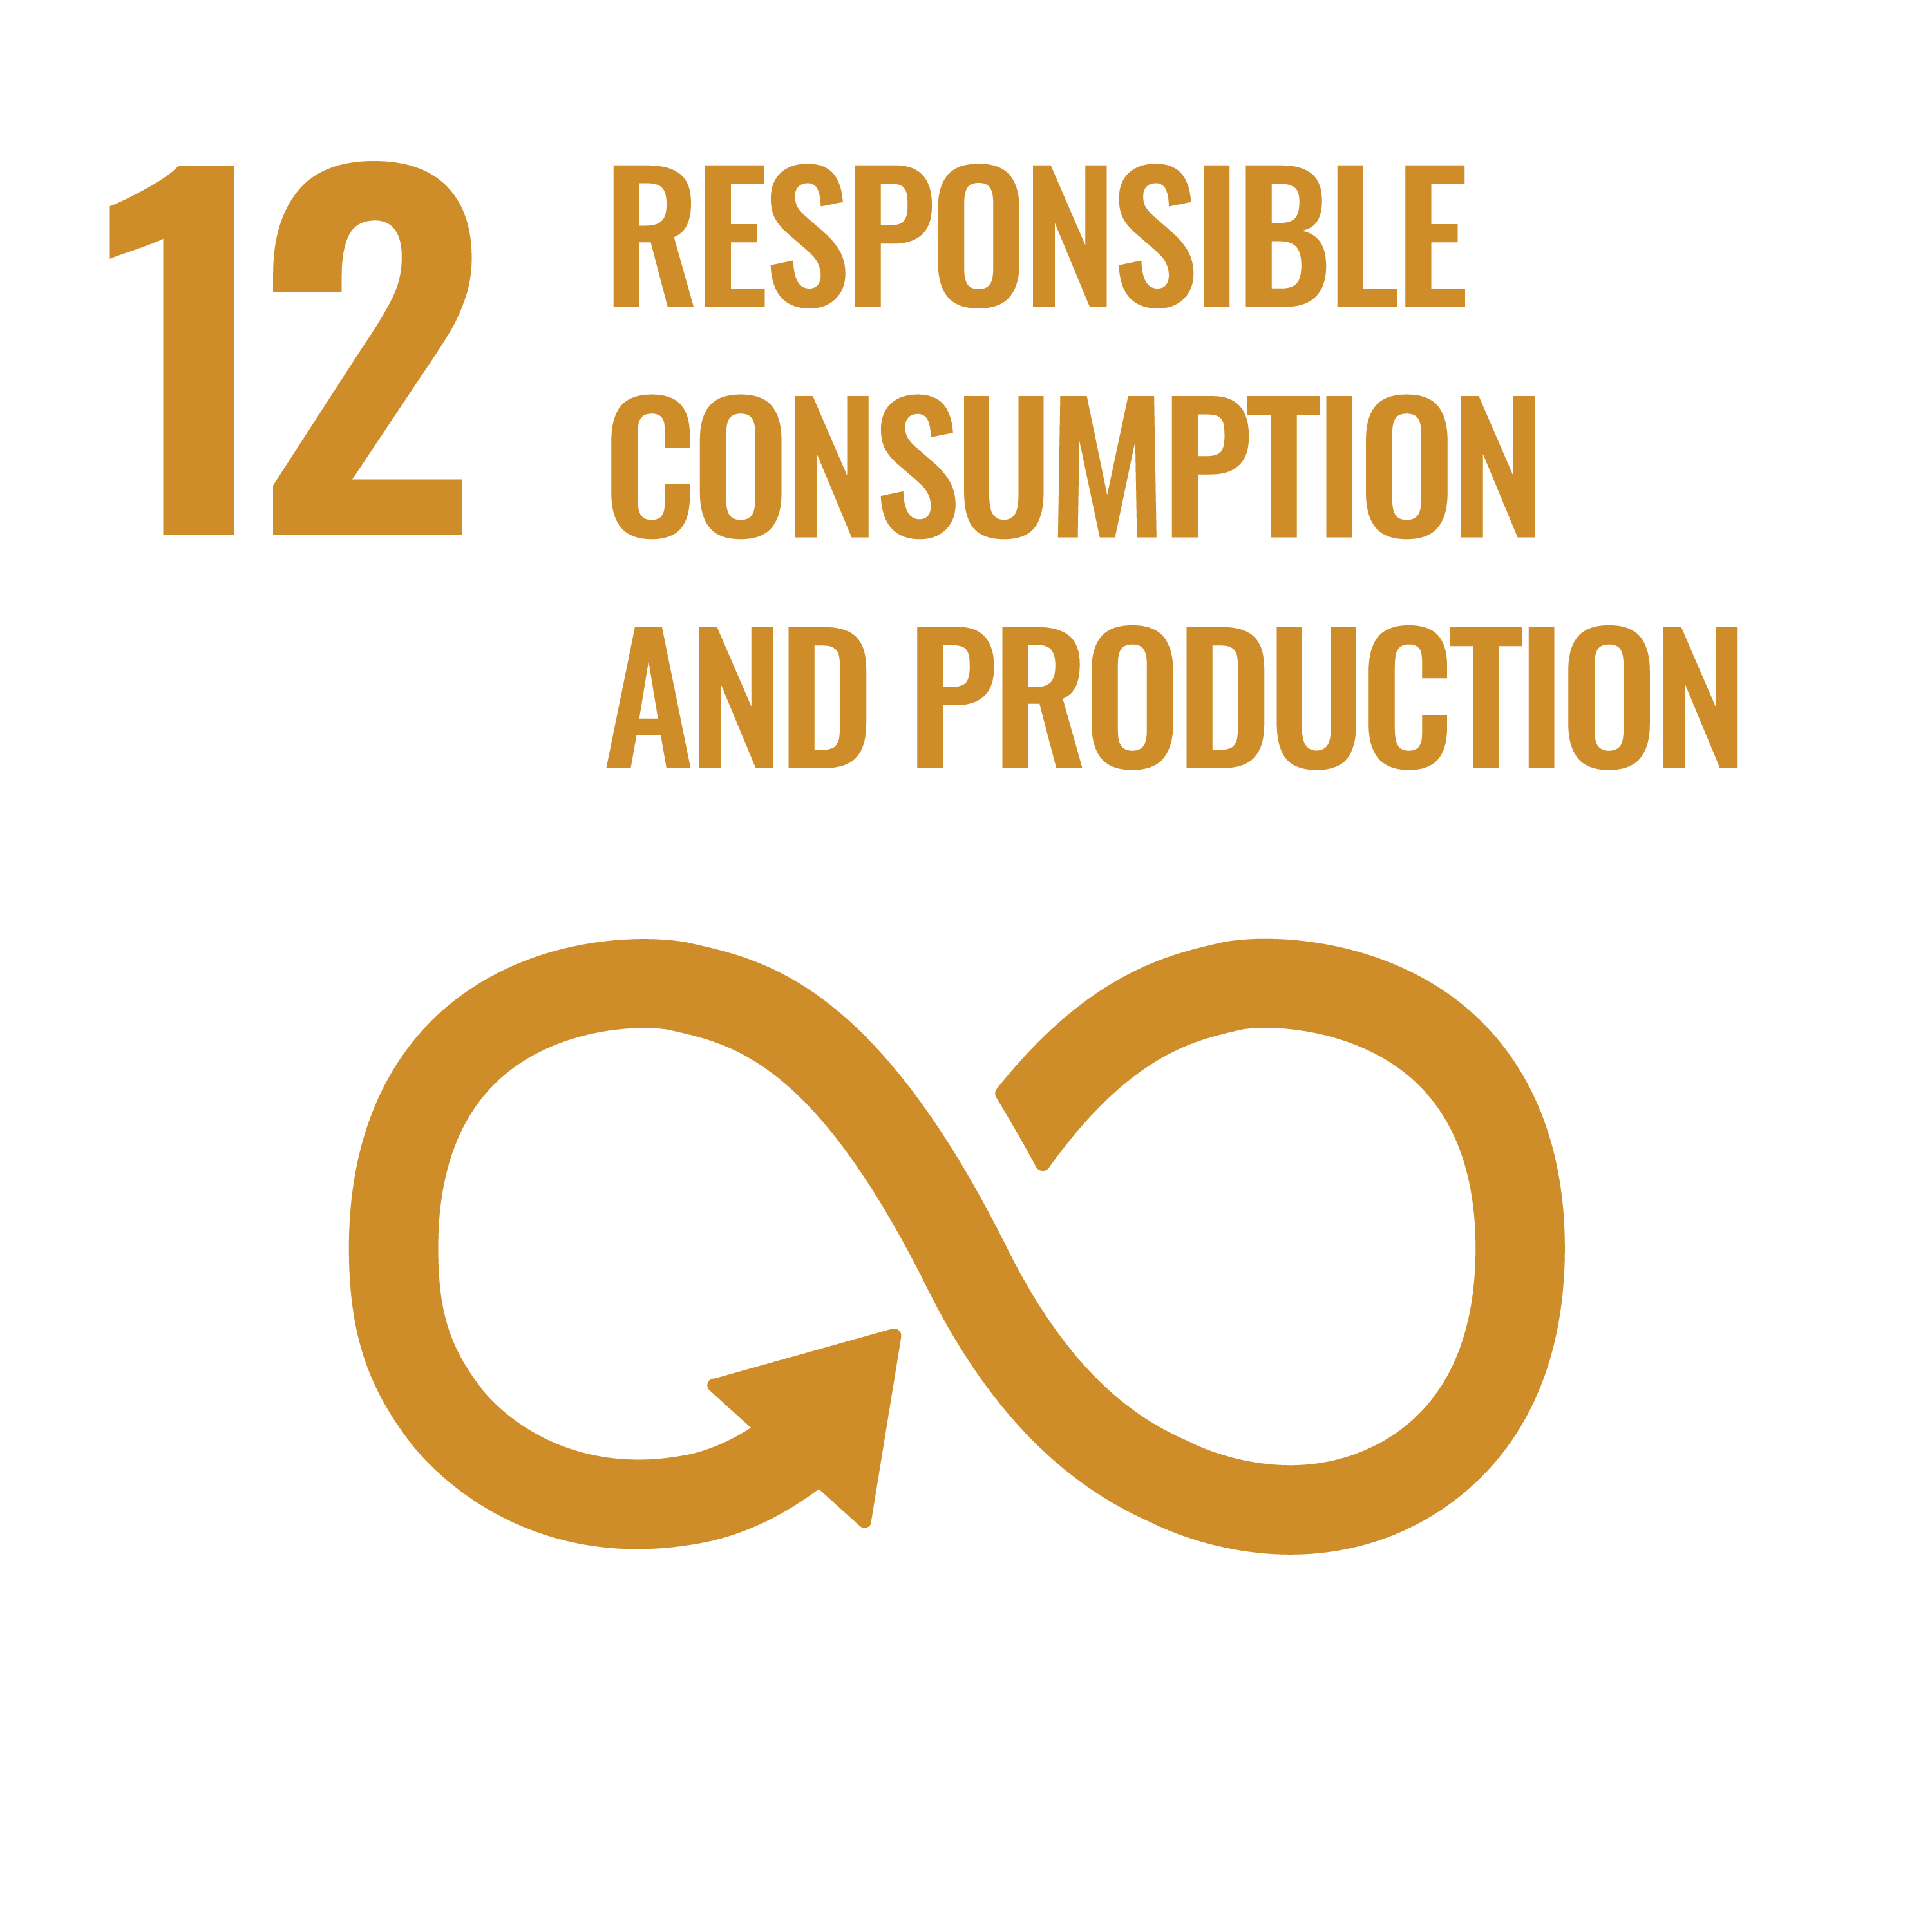
\includegraphics[width=\SDGsize]{Common/SDG_12_ResponsibleConsumption.png}~%
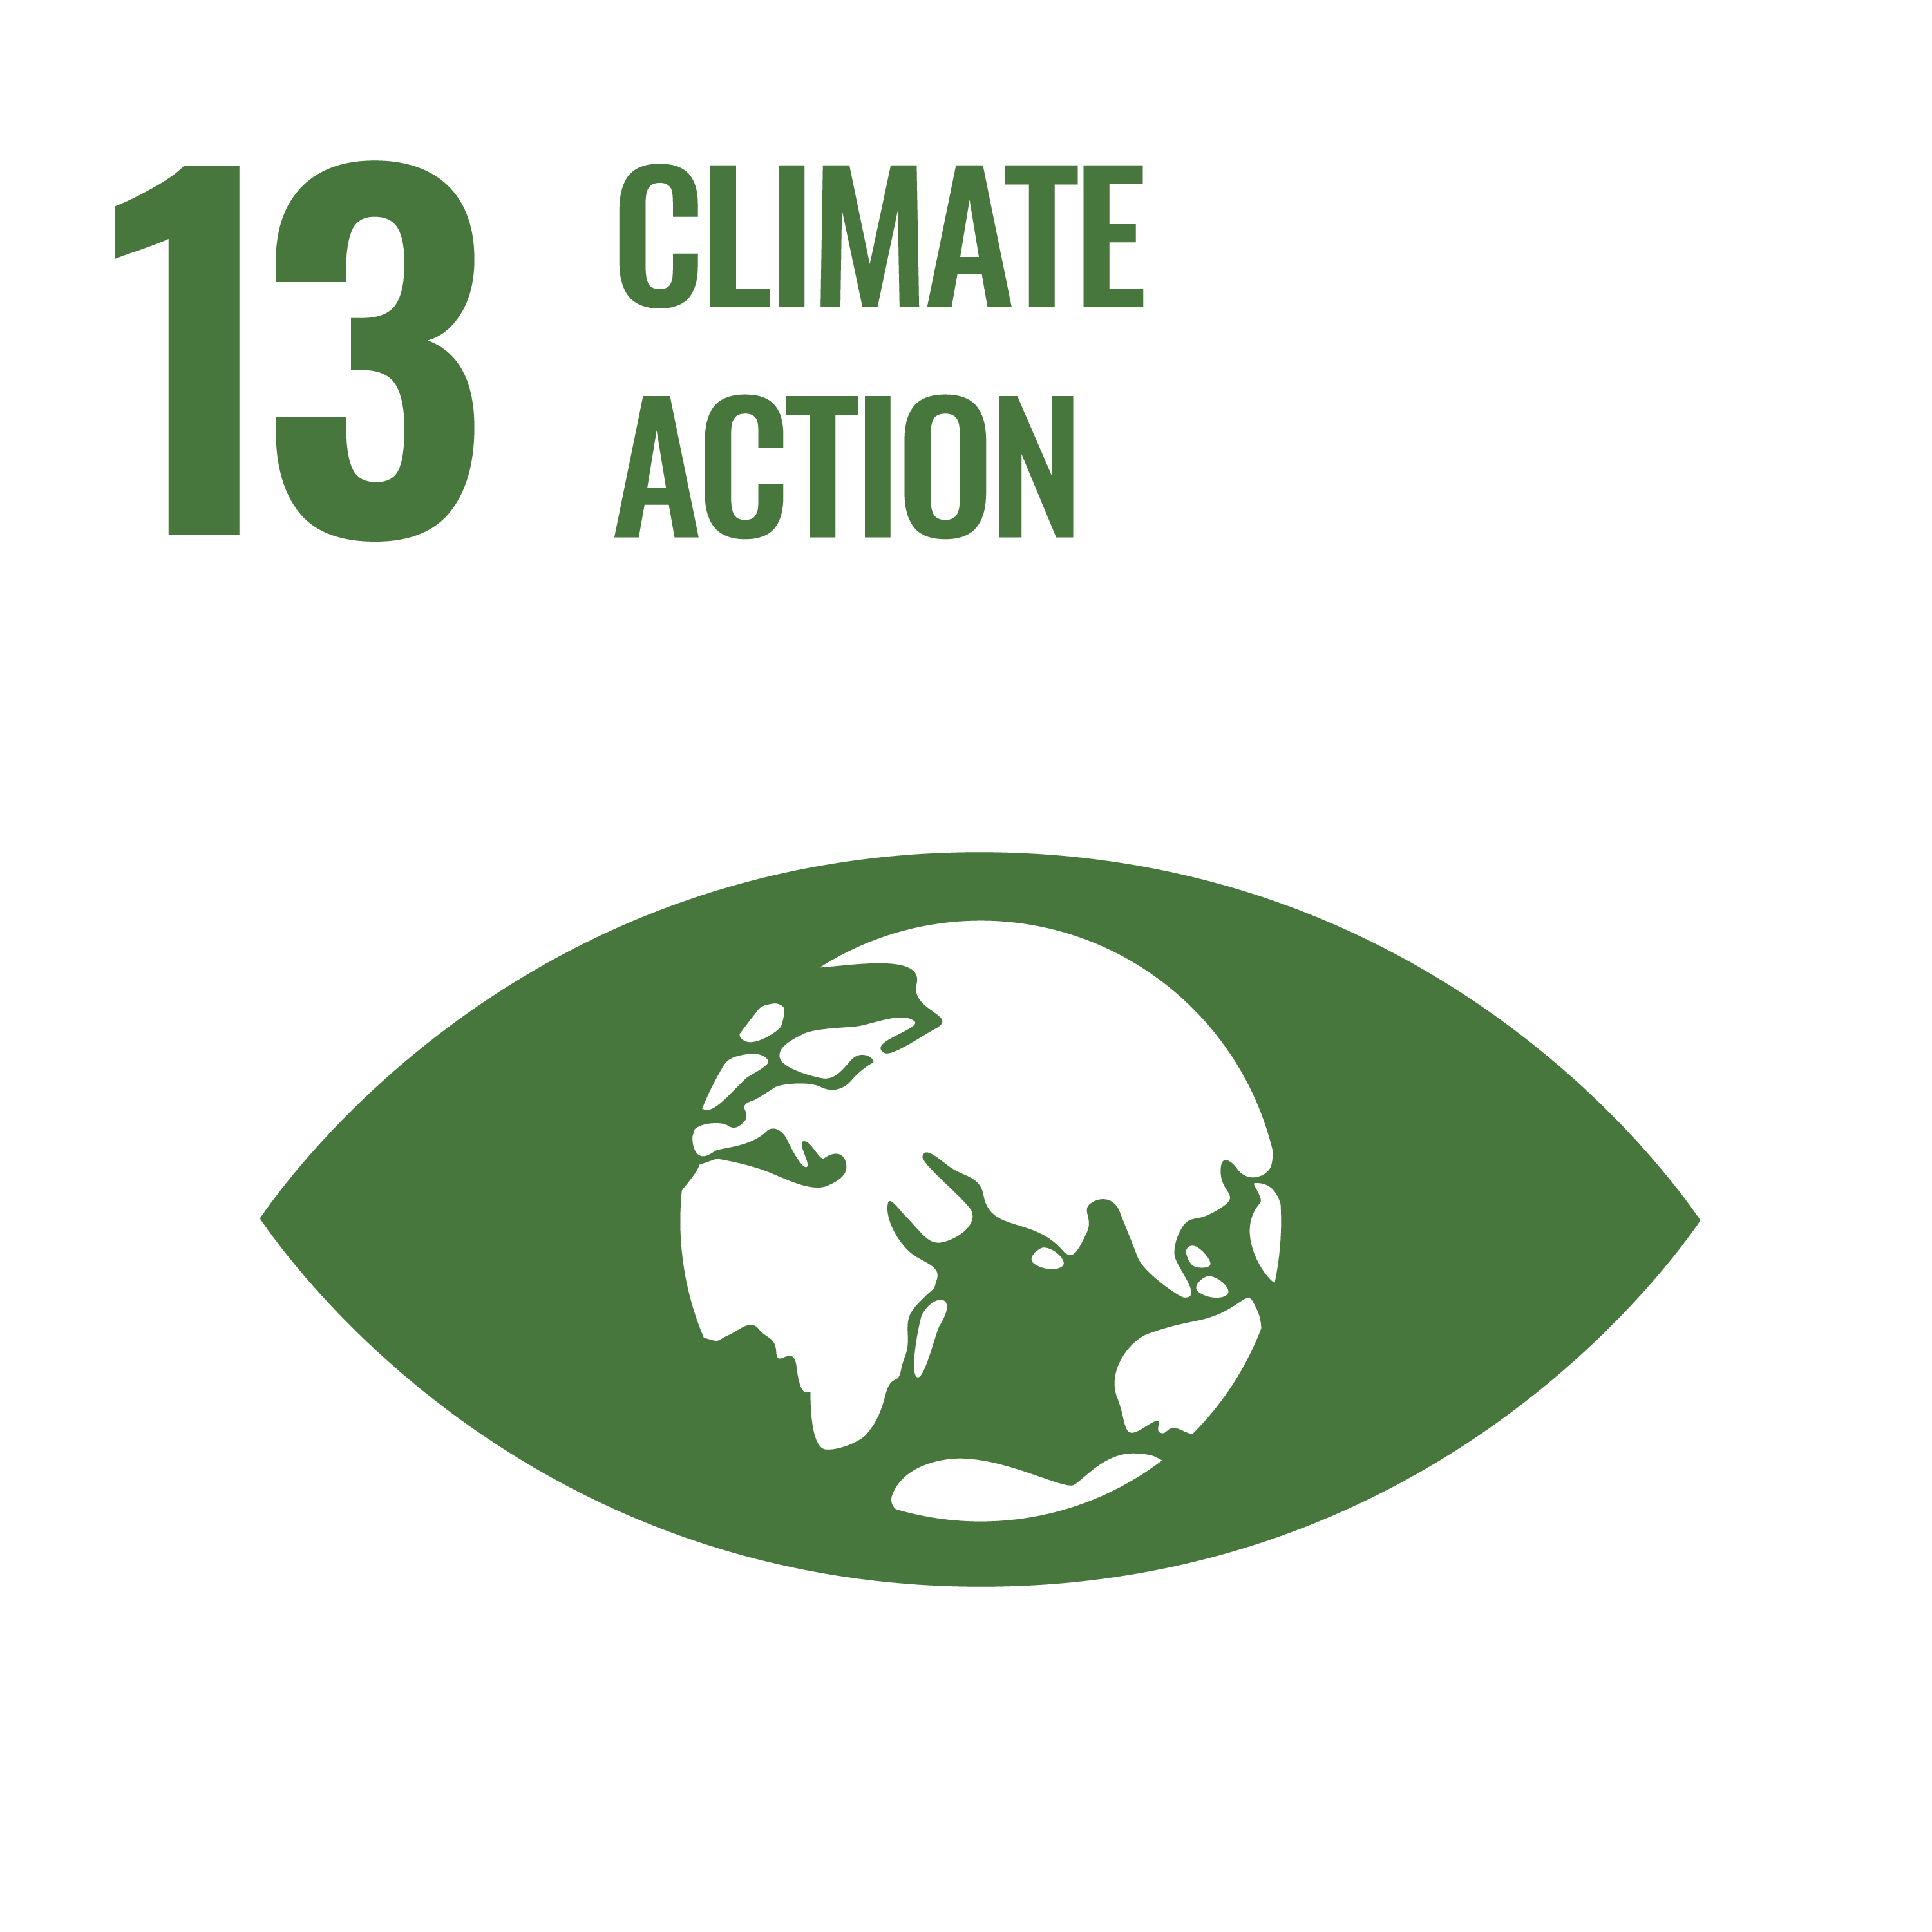
\includegraphics[width=\SDGsize]{Common/SDG_13_ClimateAction.png}~%
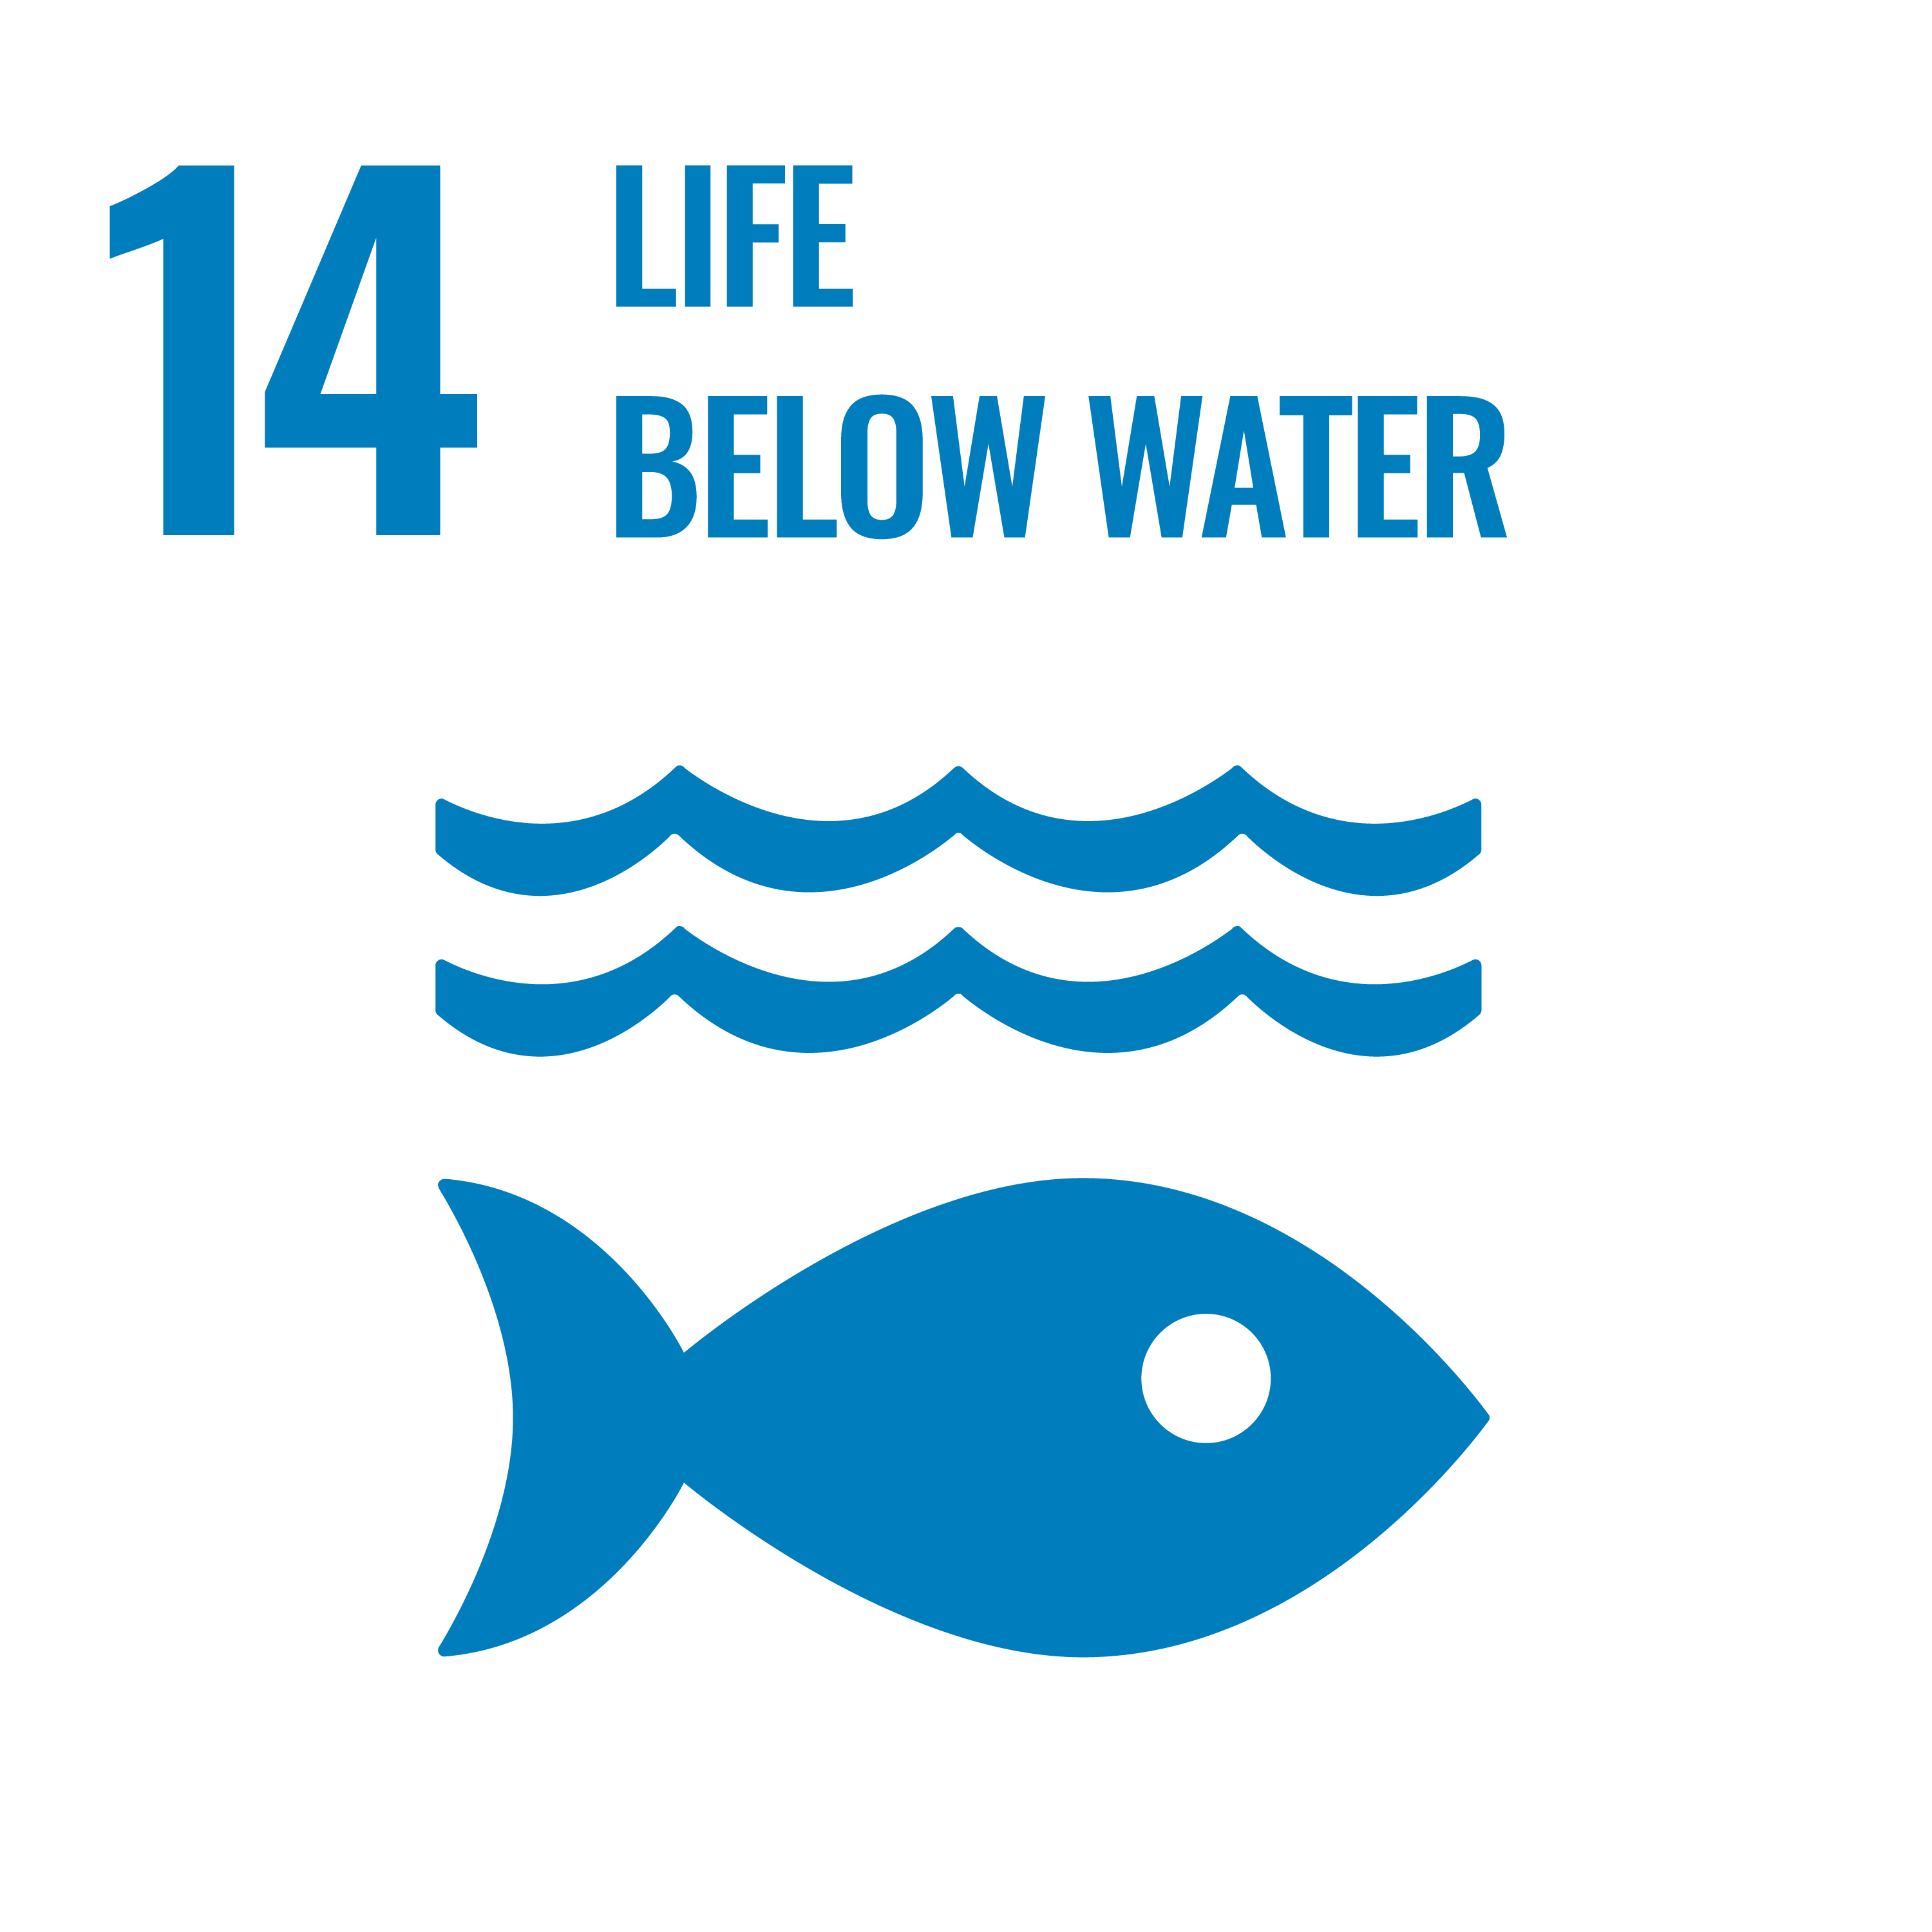
\includegraphics[width=\SDGsize]{Common/SDG_14_LifeBelowWater.png}~%
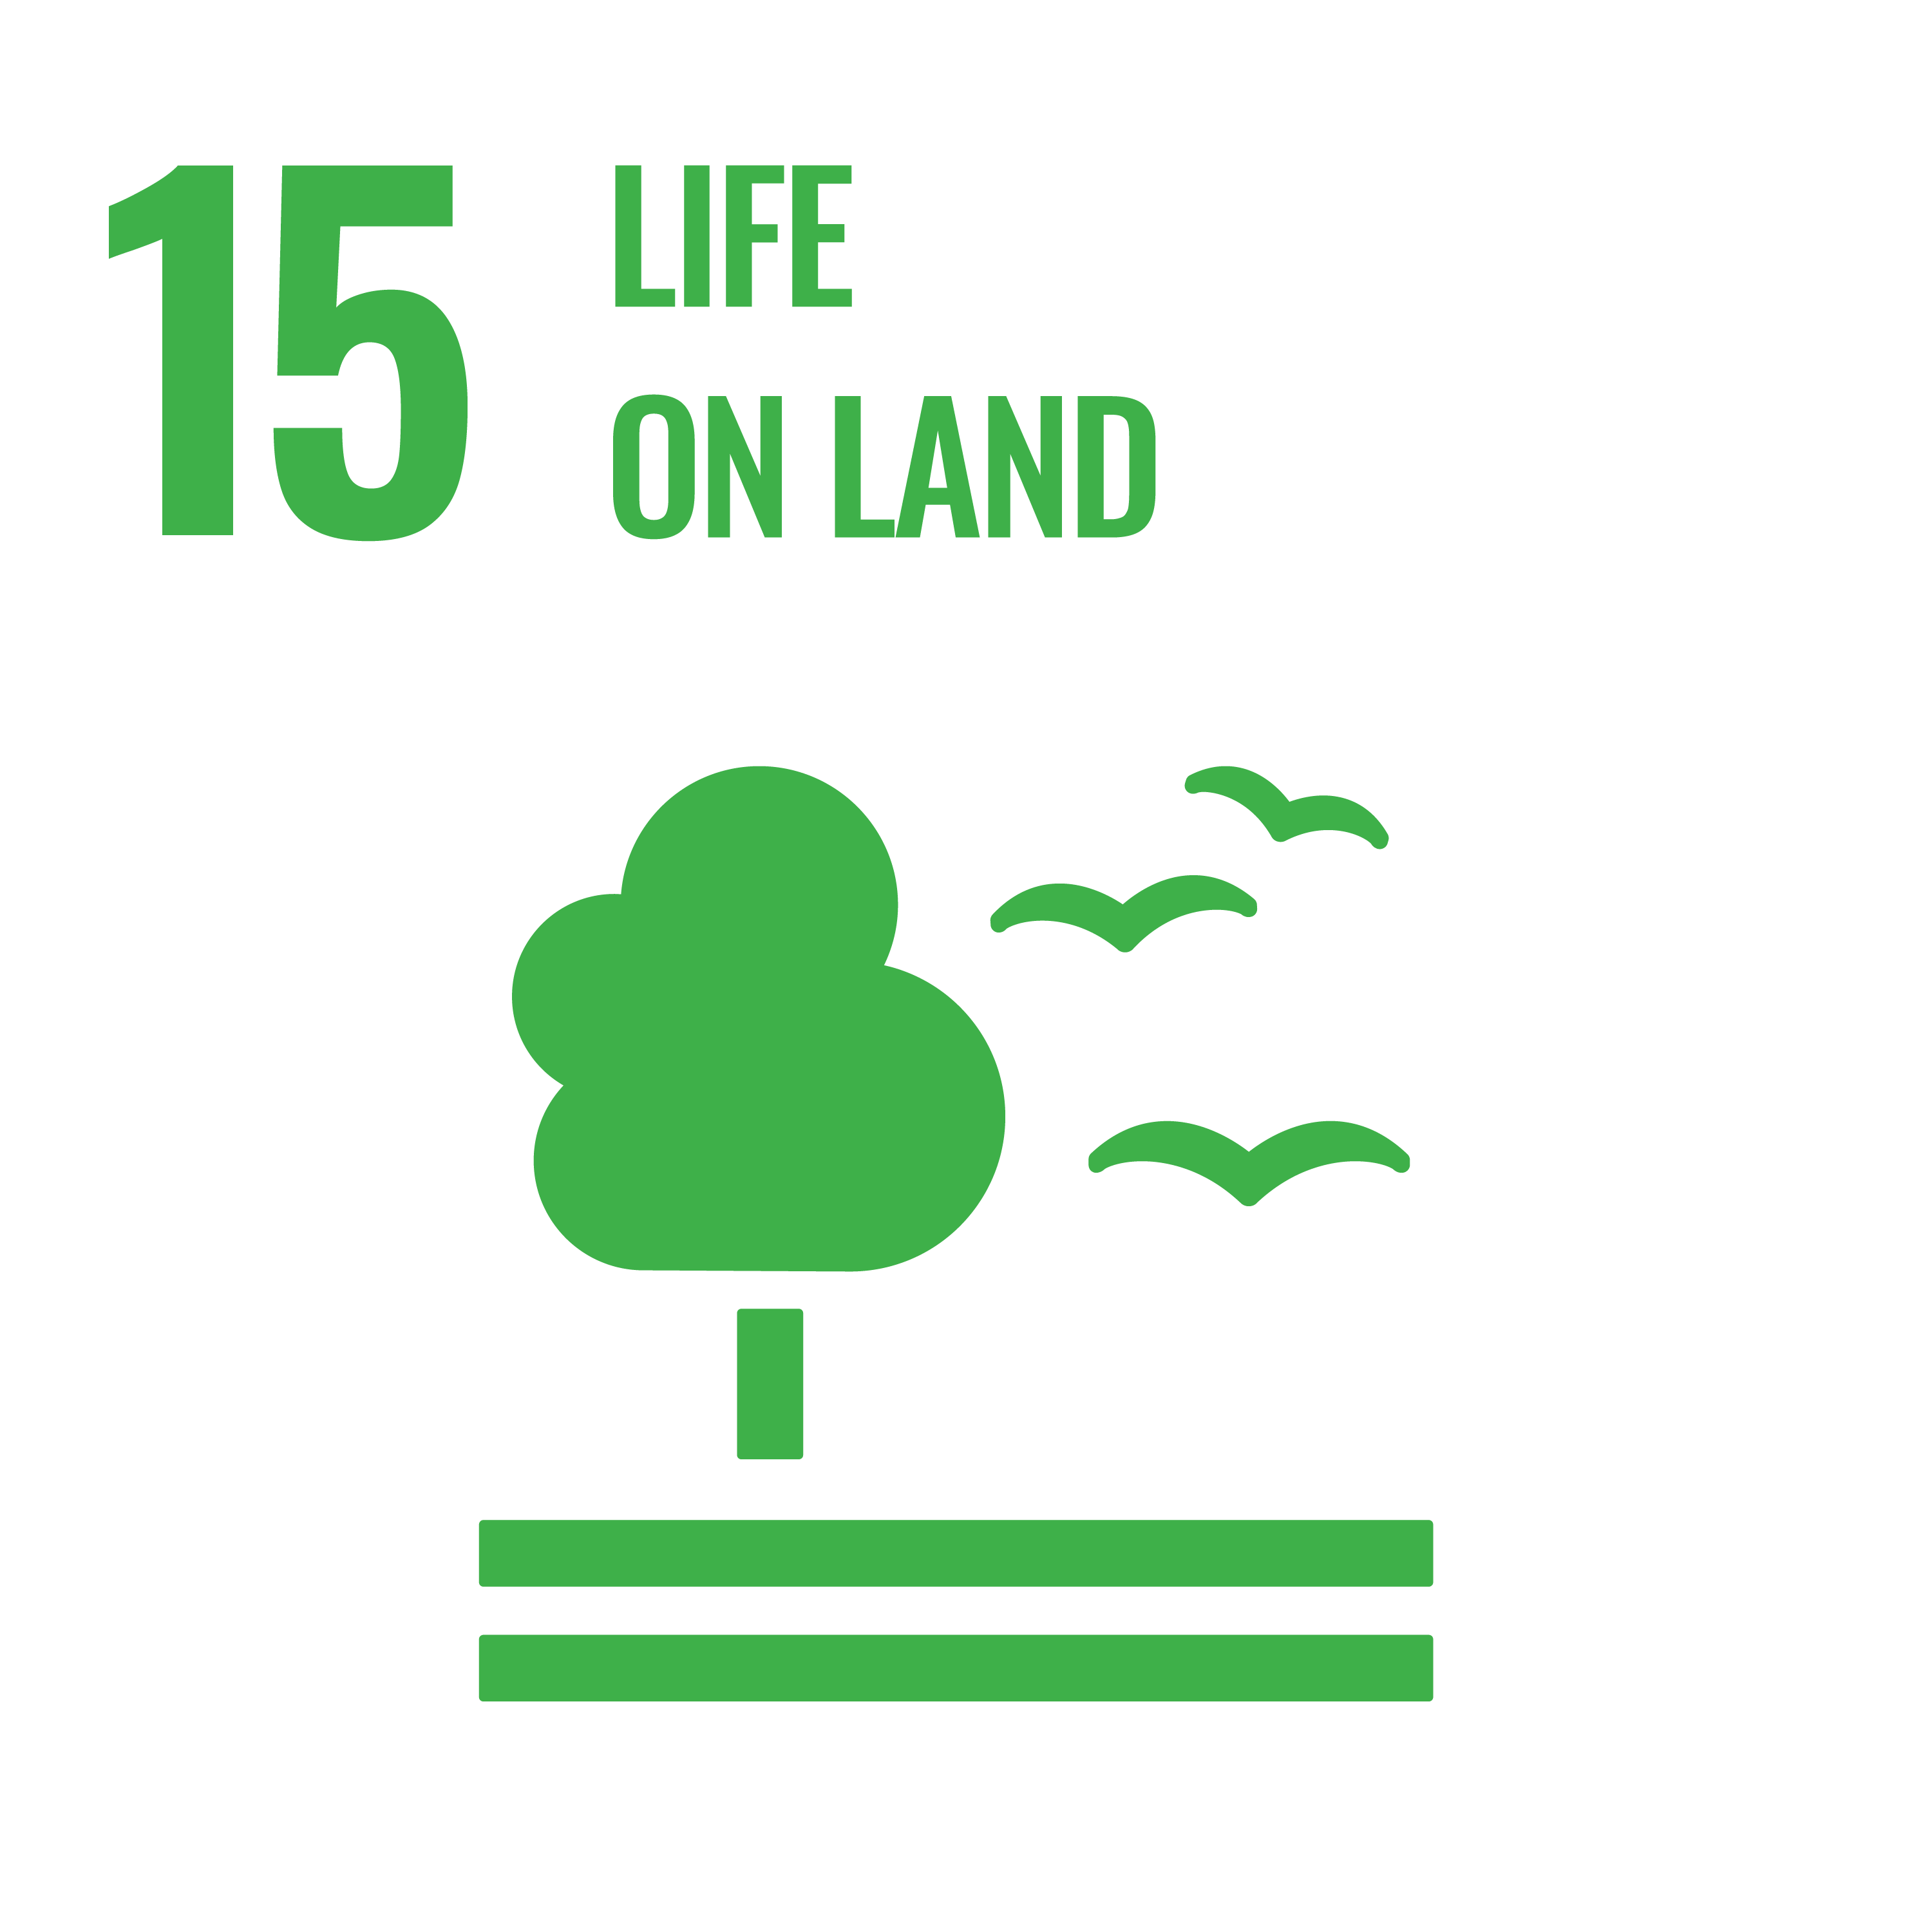
\includegraphics[width=\SDGsize]{Common/SDG_15_LifeOnLand.png}
\end{figure}

%%%%%%%%%%%%%%%%%%%%%%%%%%%%%%%%%%%%%%%%%%%%%%%%%%

\exSum

\noindent Over a quarter of global \acrshort{ghg} emissions comes from food production~\cite{USEPA}, and a quarter of this food produced is lost in the supply chain or thrown away~\cite{Searchinger2018}.  Additionally, plant and animal agriculture has extensive and profound negative impacts on the environment through land use, freshwater use and pollution, and terrestrial acidification. 

A recent article in the journal \textit{Science} argues that limiting warming to 1.5\degree C will not be possible without ``ambitious changes to food systems'' even if fossil fuel emissions are immediately halted~\cite{Clark370}.  The single most impactful measure reported in the study is a global switch to the healthy, plant-rich diet recommended by the EAT-Lancet commission \cite{WILLETT2019447}. This can be implemented immediately, and on an individual level.  Supplementing it with measures such as reducing food waste and increasing efficiencies in food production could result in a net carbon-neutral food system by 2100 \cite{Clark370}.
While sourcing sustainably-grown food and `eating local' can have a positive impact on food-related emissions (of which transportation is responsible for 6\%, see \fref{fig:food_impact}), by far the largest impact can be achieved by reducing the consumption of high-methane emitters, such as beef, lamb and dairy products~\cite{PooreNemecek2018,OWID-Sustainable,OWID-Local}.

 However, choices related to the food that we eat are deeply personal and often loaded with cultural and social significance. As such, it is important to acknowledge that changes to food systems will be a gradual process and will not have a `one size fits all' solution. Their equitable implementation will require cross-disciplinary analysis of the implications of such changes for all stakeholders. This includes producers and the local populations to which they belong, and steps must be taken to ensure communities are empowered and resilient to multiple overlapping pressures, from climate change and markets~\cite{WalshDilley2020}. The devastating impact of the quinoa boom and bust on pastoral communities in Bolivia provides one well-documented example~\cite{WalshDilley2020, Rodas2021}. Moreover, such changes must account for global disparities in wealth, and the variations in availability and access to food sources, to avoid further cementing geographic inequalities in diet. Notwithstanding the care that these factors necessitate, a significant proportion of the \ACR\ community is in the privileged position to be able to reduce their consumption of animal-derived food products and minimise food waste.

%%%%%%%%%%%%%%%%%%%%%%%%%%%%%%%%%%%%%%%%%%%%%%%%%%

\newpage
\begin{reco2}{\currentname}
{
\begin{itemize}[leftmargin=6 mm]
\item Reduce consumption of animal products, especially those that result in the highest emissions, \eg ruminant meat, and dairy.

\item Minimise, and compost, food waste.
\end{itemize}
}
{
\begin{itemize}[leftmargin=6 mm]
\item Prioritise plant-based options in conference catering, and optimise service method to reduce food waste.
\end{itemize}
}
{
\begin{itemize}[leftmargin=6 mm]
\item Incentivise the consumption of plant-based products at on-site restaurants by increasing their variety and quality,  and subsidising their cost.

\item Highlight the environmental impact of food choices through service layout and labelling.

\item Minimise food waste by providing multiple portion sizes and donating unused food.

\item Read section on waste (Section~\ref{sec:Waste}) and limit food-service waste \eg through industrial composting of biodegradable food containers.
\end{itemize}}
\end{reco2}

%%%%%%%%%%%%%%%%%%%%%%%%%%%%%%%%%%%%%%%%%%%%%%%%%%
\newpage
\subsection{Food Production\label{sec:agriculture}}

\begin{figure}
    \centering
    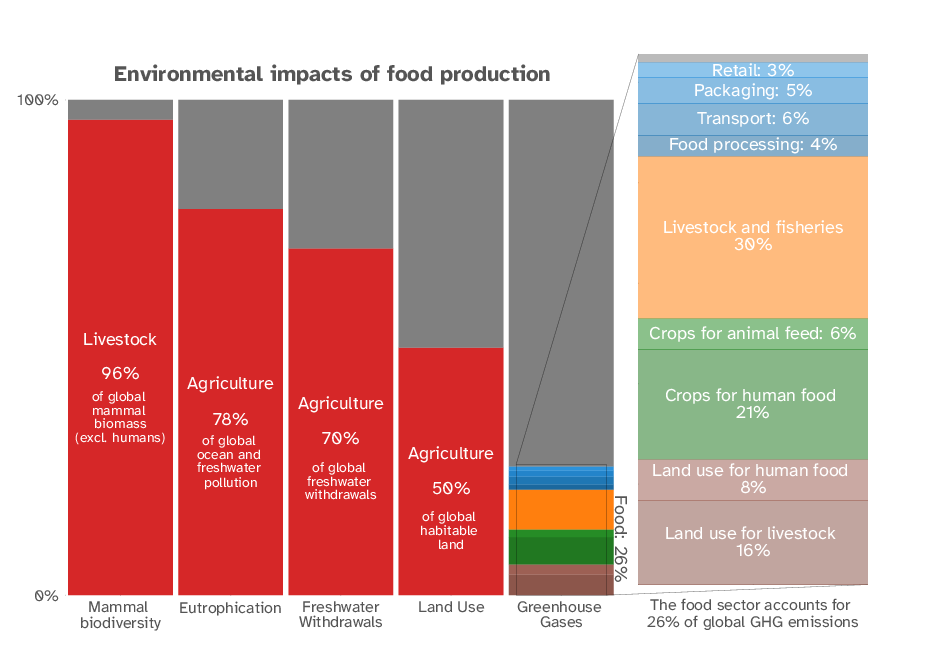
\includegraphics[width=\textwidth]{Sections/Figs/Food/FoodEnvironment.png}
    \caption[Environmental impact of food production]{ Environmental impact of food production, with fine-grained partitioning of GHG emissions by food sector. Figure modified from Ref.~\cite{OWID-Food}, based on data from Refs.~\cite{PooreNemecek2018} and~\cite{Bar-On6506}.
    \label{fig:food_impact}}
\end{figure}

\fref{fig:food_impact} reveals the overall environmental impact of food production.  The agriculture sector uses 70\% of the world's fresh water reserves and has caused eutrophication\footnote{Excessive fertilizer runoff to freshwater environments causing algal blooms, oxygen depletion, and fish die-offs.} of most of the world's oceans and freshwater.  It is responsible for large-scale deforestation and habitat loss~\cite{OWID-Food, PooreNemecek2018, Xu2021}, resulting in an historic low in mammalian biodiversity, with total mammal biomass dominated by humans and their livestock \cite{Bar-On6506}. 

Animal agriculture is responsible for just over half  of GHG emissions from the food sector, due to direct emissions from livestock and fisheries, land use, and production of crops for animal consumption.\footnote{Organic animal-derived foods often have higher yields of GHG emissions, partly because of the animals' lower productivity~\cite{Pieper2020}.}  It accounts for three-quarters of global agricultural land use, while providing just a fifth of the world's calories, and under 40\% of its protein supply~\cite{OWID-Food, PooreNemecek2018, Xu2021}.  The over-use of antibiotics in animal agriculture is partially responsible for the development of antimicrobial resistance in "superbugs"~\cite{AMBR2005}, and may be a risk factor for the emergence of new zoonotic diseases~\cite{Jones8399, Espinosa, Morand}.  Furthermore, there is substantial evidence linking high intake of red meat to an increased rate of heart disease~\cite{meat-health}.

Shifting consumption away from animal products to a more plant-based diet would significantly reduce both the environmental and healthcare costs of food systems.  
The potential annual reduction in GHG emissions from eliminating different food groups from our diet is shown in \fref{fig:foodchanges}.  
Beef, lamb, and dairy, responsible for the largest cumulative global emissions, are also among the highest emitters per 100 grams of protein, see \fref{fig:ghg-per-protein}.  In addition, animal products are generally more expensive than plant products~\cite{Springmann2021}, as well as being less inclusive of people with dietary restrictions or preferences due to religion, lifestyle choices, or certain food allergies or intolerances.

%%%%%
\begin{figure}[htb]
    \centering
    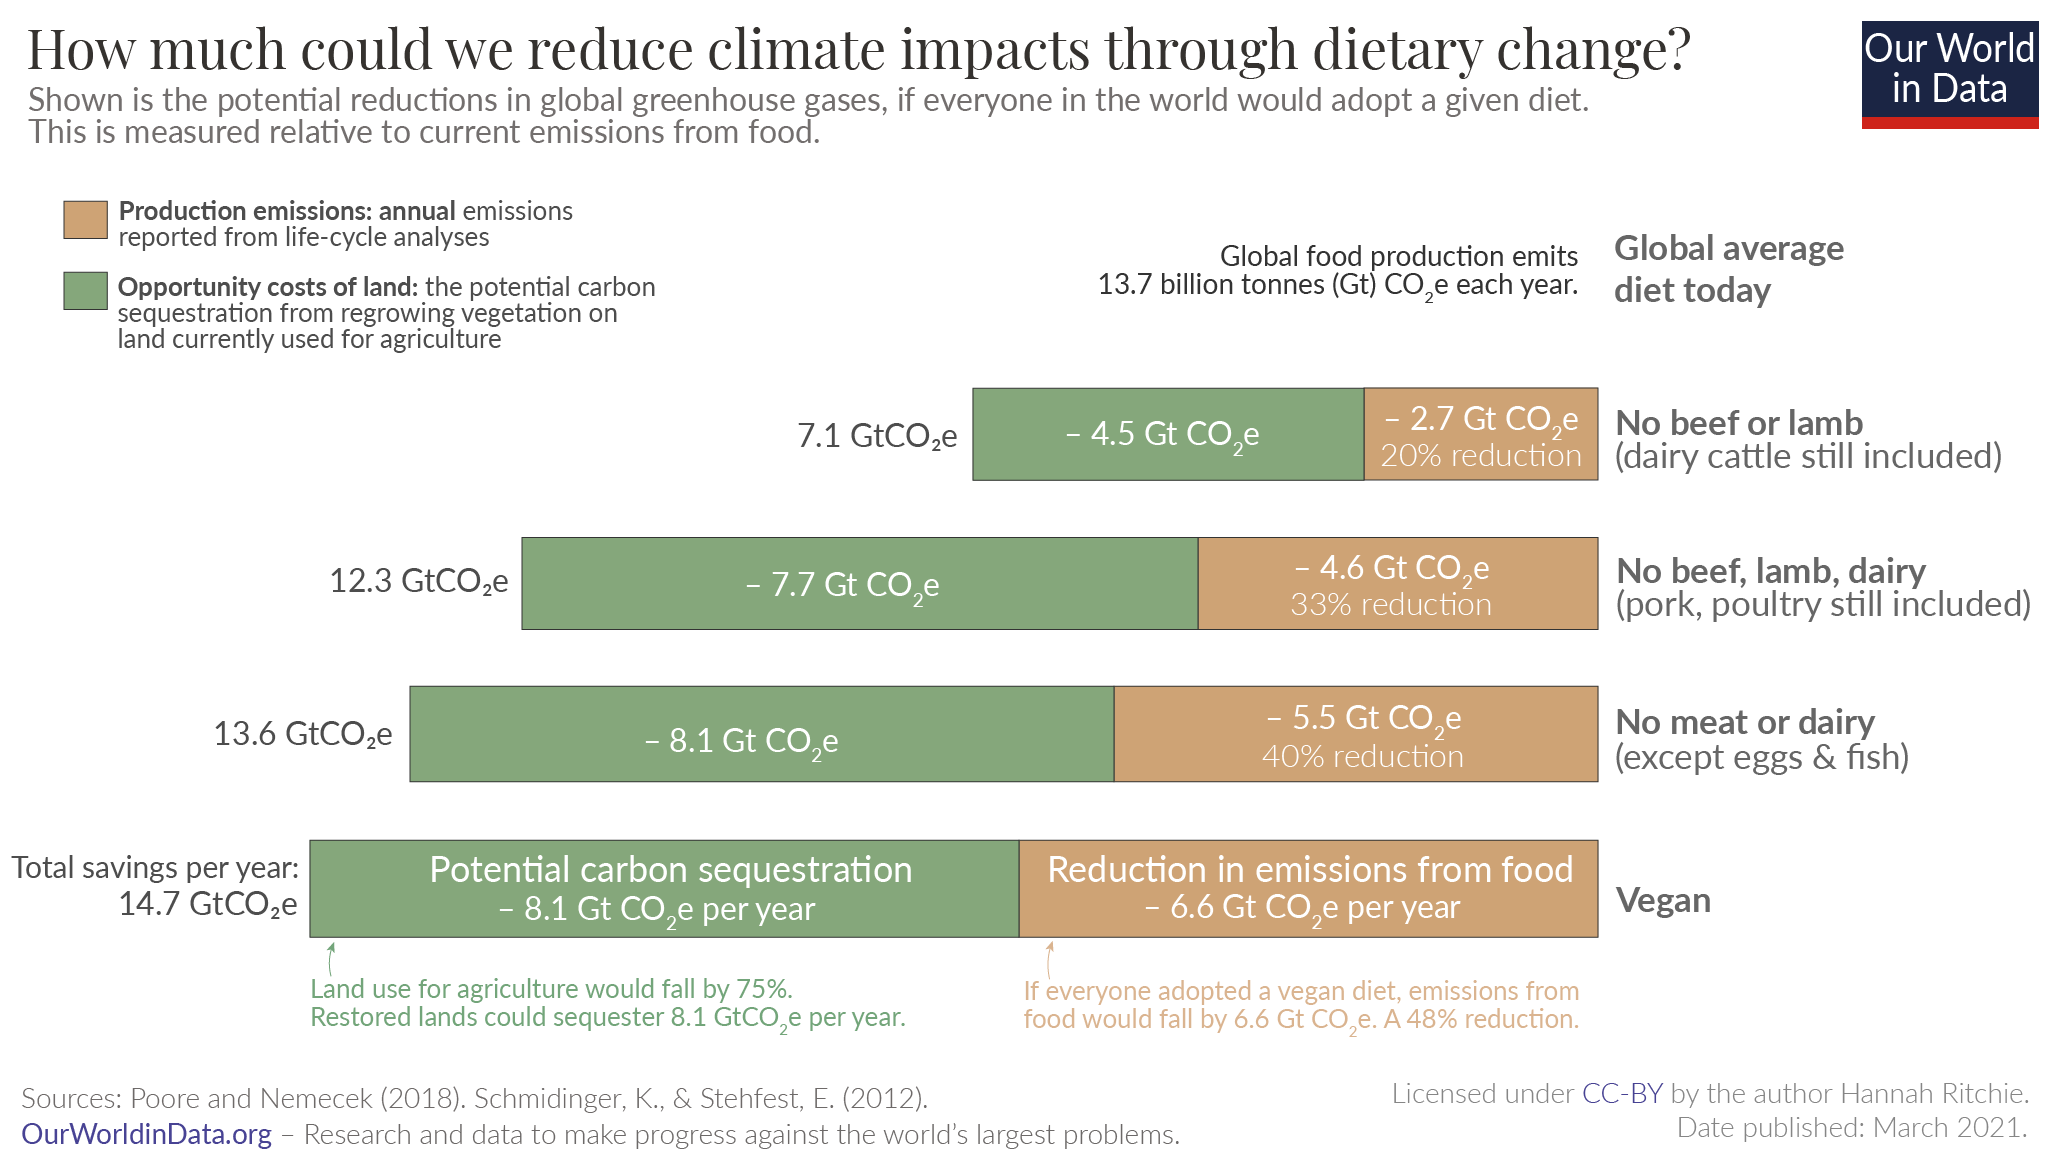
\includegraphics[width=0.9\textwidth]{Food/CarbonSavingsDiet.png}
    \caption[Annual carbon opportunity due to changes in diet.]{Potential reduction in GHG emissions due to changes in diet, relative to current emissions from food.  Figure reproduced from Ref.~\cite{OWID-CarbonOpportunity}, based on data from Refs.~\cite{PooreNemecek2018,Schmidinger}.
    \label{fig:foodchanges}}
\end{figure}

%%%%%%%%%%%%%%%%%%%%%%%%%%%%%%%%%%%%%%%%%%%%%%%%%%

\subsection{Food Service}

Several universities and other institutes for higher education have implemented measures to limit or eliminate consumption of animal-derived foods and reduce food waste, including eliminating red meat from their cafeterias, increasing the quality and variety of plant-based options, changing the cafeteria layout, and modifying default meal options and food labelling~\cite{Berlin, EPFL, Cambridge, Goldsmiths}.    By way of illustration, we quantify the GHG savings due to replacing beef with alternative sources of protein in the weekly menu of CERN Restaurant 1 in \csref{case:CERNR1}.

At conferences and workshops, the primary purpose of any food served is to create additional opportunities for attendees to mingle and discuss.  As such, conference organisers enjoy more leeway to make sustainable food choices the default option for these short-term, small-scale events.  \bpref{catering_bp} contains two examples of successful physics conferences with plant-based catering. They highlight, among other things, the importance of institutional partnerships with plant-friendly caterers, and organisers should push for these if they do not already exist.  For further discussion on sustainability at conferences, see Section~\ref{sec:ConferenceWaste}.

\begin{casestudy}[Sustainable catering at CERN Restaurant 1\label{case:CERNR1}]{Sustainable catering at CERN Restaurant 1}%
    CERN Restaurant 1 (R1) serves an average of 2,000 meals per day~\cite{CERNACCUMeeting}. It offers five hot meal options daily, and has recently overhauled its menu options to include a larger variety of vegetarian and plant-based options, including at least one plant-based main course.  We assume each of the five mains are chosen with equal likelihood, and neglect cold food options, such as salads and sandwiches.

    \begin{figure}
        \captionsetup{type=figure}
        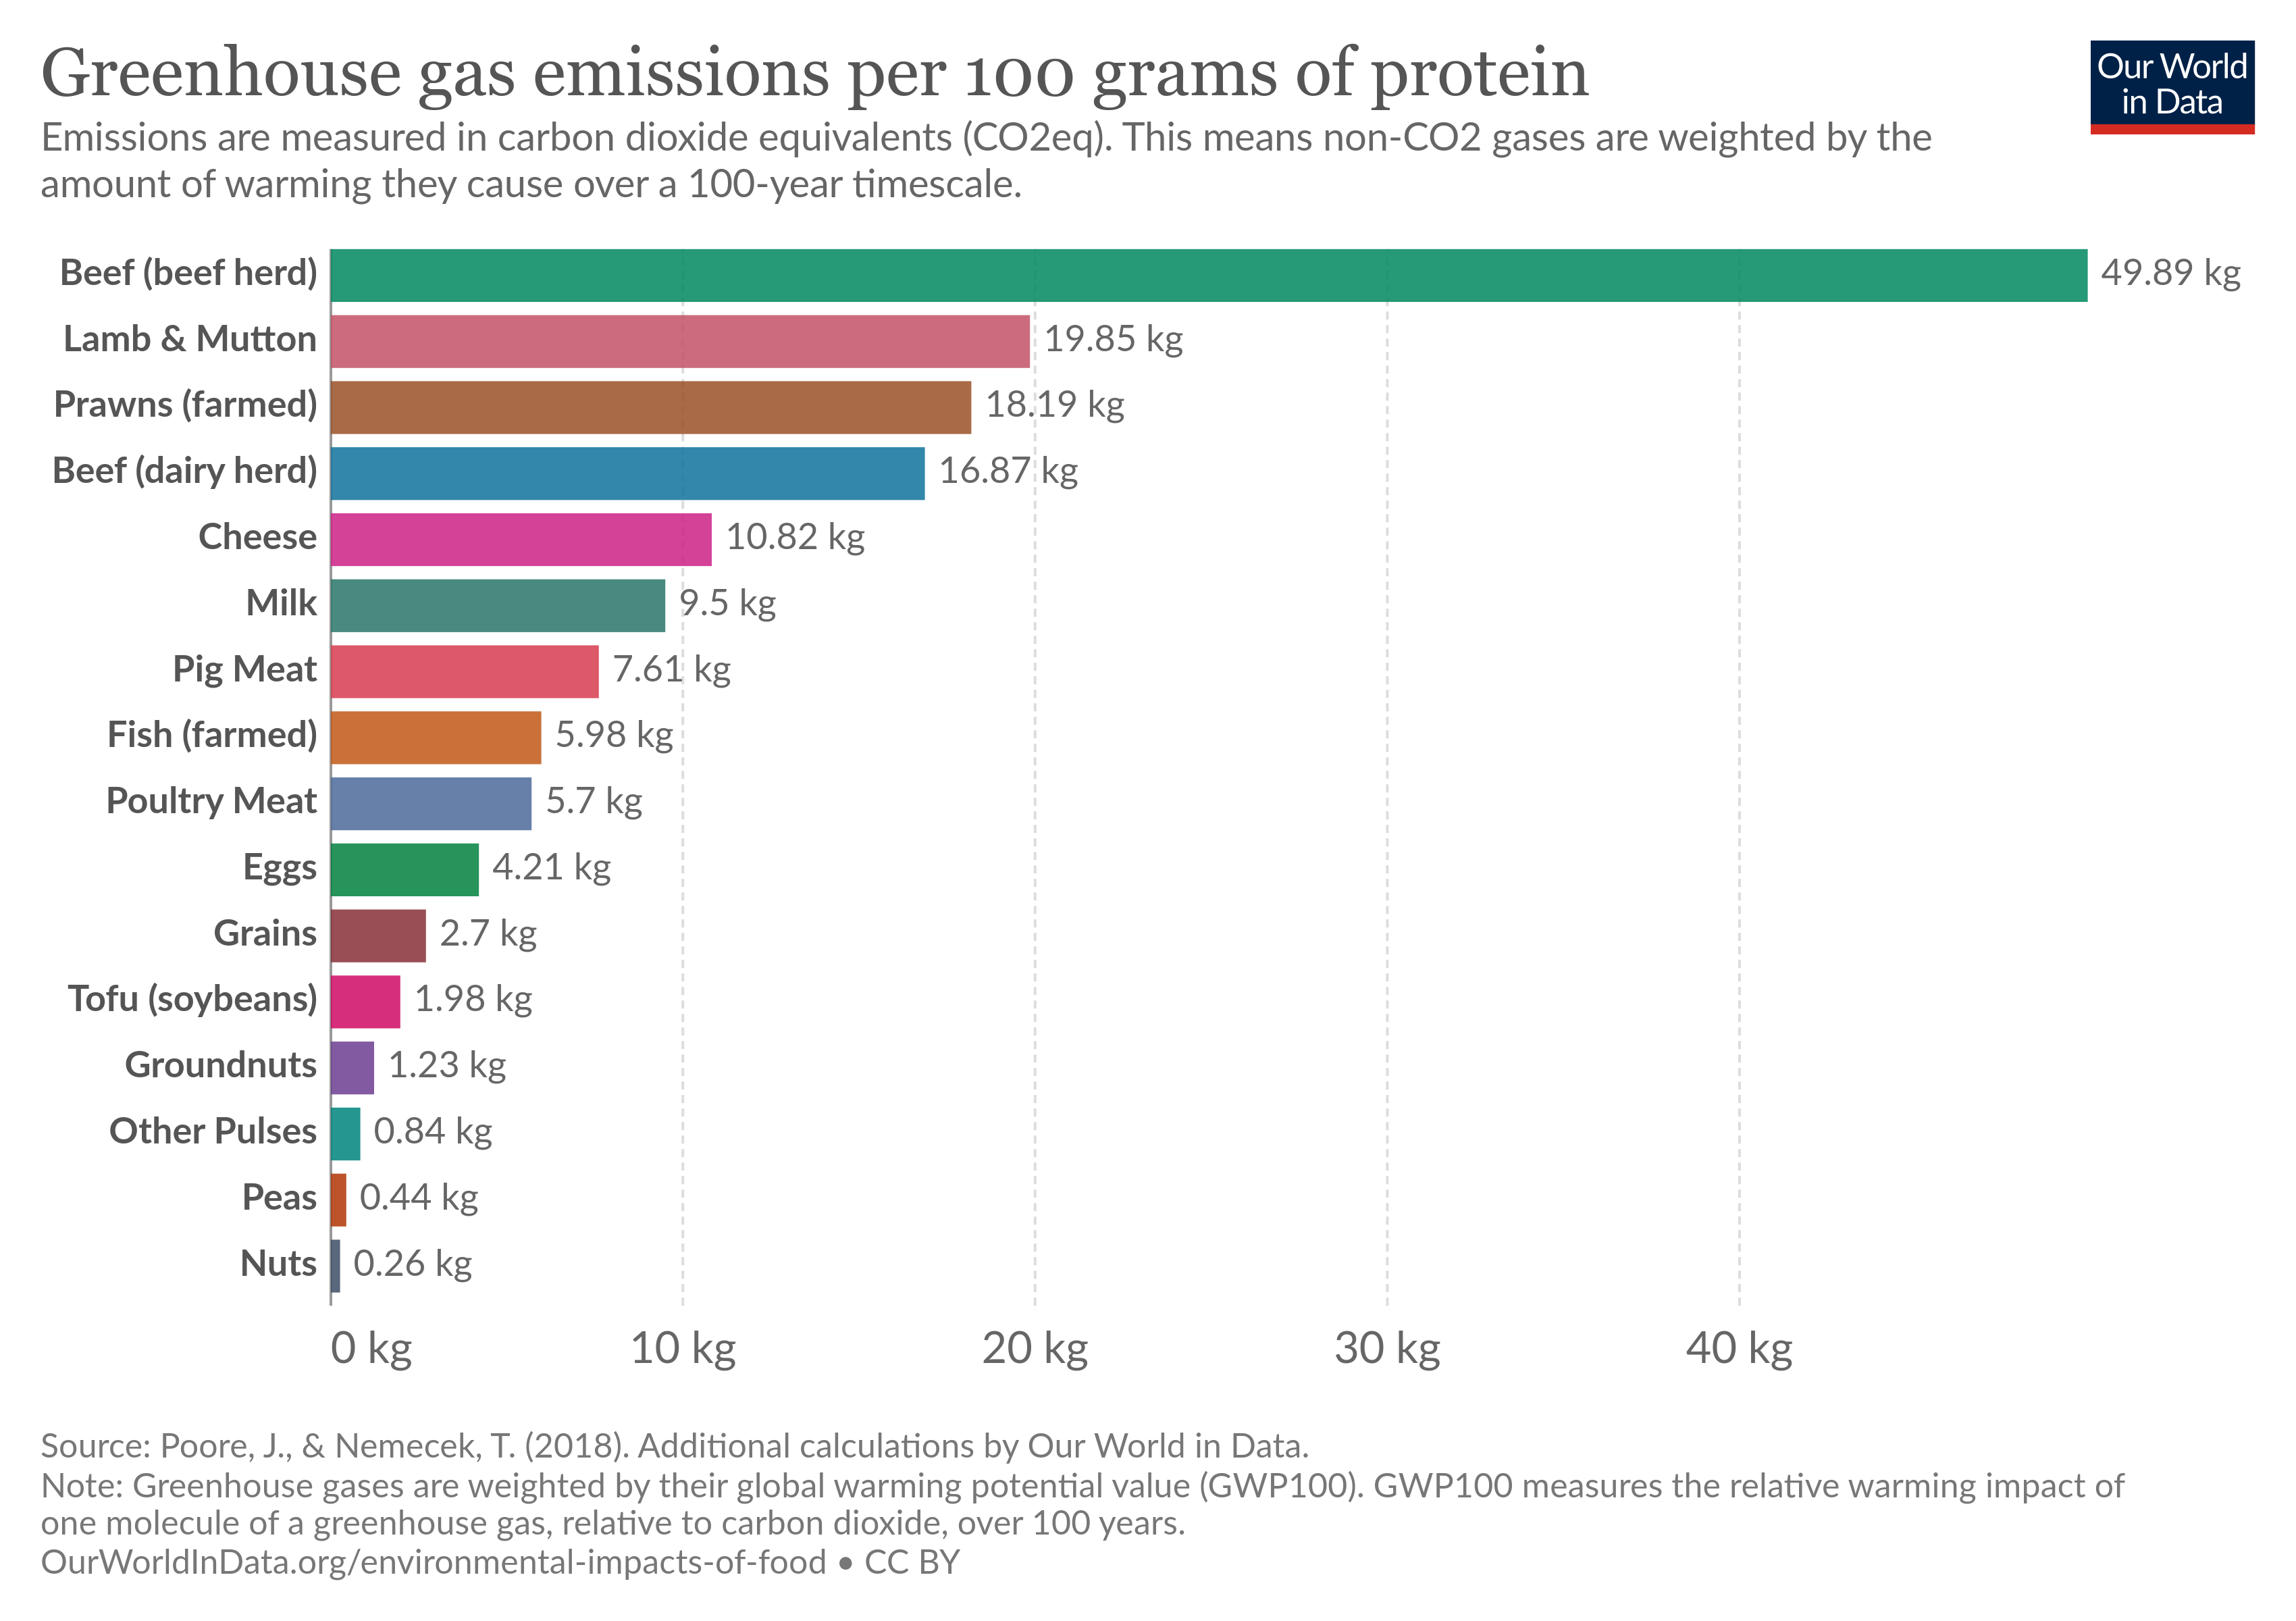
\includegraphics[width=0.85\textwidth]{Sections/Figs/Food/Emissions-protein.png}
        \caption[GHG emissions per 100 g of protein]{GHG emissions in \CdOe\ per 100 g of protein. Figure reproduced from Ref.~\cite{OWID-Food}, based on data from Ref.~\cite{PooreNemecek2018}.}
        \label{fig:ghg-per-protein}
    \end{figure}

    In, \eg the week beginning 27 June 2022, beef, fish and seafood were each served three times as the primary component of the meal, veal once, poultry five times, and fish twice.  We assume that these distributions are representative of a typical weekly menu at R1 and that the beef originated from beef-herd cows. The GHG emissions of the various forms of protein are shown in \fref{fig:ghg-per-protein}.

    Substituting each gram of protein from beef with a gram of protein from chicken or fish reduces emissions by 440~g \CdOe.  
    Assuming a serving contains 20~g of protein\footnote{The Mayo Clinic recommends 15--30~g of protein per meal~\cite{MAYO}.}, substituting all beef meals at R1 with farmed fish or chicken would result in a reduction of its annual carbon footprint by 528 \tCdOe.\footnote{Substituting 1,200 beef meals weekly over 50 weeks, each meal consisting of 20~g protein, with chicken or fish leads to a reduction of $1,200\times 50\times 20\times 0.440$ kg \CdOe \; in emissions. Note however that farmed chicken and fish give rise to significant environmental impacts in sectors other than GHG emissions~\cite{KUEMPEL2023}.  The estimated emissions overshoots CERN's reported 2019 beef-related emissions by a factor of two \cite{HSENote}.  The reason for this discrepancy is unclear, since details of the calculation from Ref.~\cite{HSENote} were not shared.}
    This corresponds to approximately  260 return flights between London and New York. 
    Both the emissions savings and the overall environmental impact would be even greater if plant-based substitutions were made.

    Instituting one weekly meat-free day (taking as a benchmark a day where one beef, one fish, and one poultry meal were served, and replacing them with one tofu-based meal and two pulse-based meals) would result in a reduction of 735 \tCdOe\ annually, where the bulk of the savings comes from the beef replacement.
\end{casestudy}

\begin{bestpractice}[Plant-based catering at conferences and workshops\label{catering_bp}\\
{\footnotesize\noindent We thank Hannah Wakeling (for WIP 2019) and Stefan Fredenhagen (for YRISW 2019) for sharing their experience as part of the respective organisational teams.}]{Plant-based catering at conferences and workshops}%
\noindent The conference Women in Physics 2019~\cite{WIPC} at McGill University in Montréal was designed as a `sustainable' conference. Ecologically-friendly choices were made by offering purely plant-based catering, sustainable goodie bags, and use of reusable tableware (see also Section~\ref{sec:CateringTableware}). Most of the feedback regarding these measures was positive. An important point for the organisers was to advertise the catering as sustainable, and not only as vegan, since according to their experience this ``helped the way the catering was received'' by the participants. The organisers mentioned that it can be difficult to find a vegan caterer if the only choices are partners of the university hosting the conference, but it was nevertheless possible in their case.\\

   The `Young Researchers Integrability School and Workshop (YRISW) 2019: A modern primer for 2D CFT'~\cite{YRISW} in Vienna offered only plant-based catering. The organizers of the school selected this option as the ``most inclusive approach'', where people are not separated according to their eating habits. They wanted to advertise plant-based food to the participants, and "reduce the environmental impact of the event". The limited food options also reduced the total cost of the catering. The organisers received positive feedback, not only for the food itself but also for the ``effort to reduce the ecological impact of the school". The organizers emphasised the importance of finding a specialist plant-based caterer to ensure the quality and flavour of the food.
\end{bestpractice}

\end{document}